\documentclass[UTF8,a4paper,11pt,fontset=fandol,scheme=plain]{ctexart}
\usepackage[margin=23mm,headheight=14pt]{geometry}
\usepackage{amsmath,amssymb,bm,graphicx,booktabs,tabularx,array,caption,float,placeins}
\usepackage{xcolor,enumitem,fancyhdr}
\usepackage[unicode,colorlinks=true,linkcolor=black,citecolor=black,urlcolor=blue!45!black]{hyperref}
\setmainfont{texgyretermes-regular.otf}[BoldFont=texgyretermes-bold.otf,ItalicFont=texgyretermes-italic.otf,BoldItalicFont=texgyretermes-bolditalic.otf]
\setlength{\parindent}{0pt}
\setlength{\parskip}{5pt}
\linespread{1.18}
\setlength{\emergencystretch}{2em}
\setlength{\textfloatsep}{10pt}
\raggedbottom
\renewcommand{\topfraction}{0.95}
\renewcommand{\bottomfraction}{0.85}
\renewcommand{\textfraction}{0.05}
\renewcommand{\floatpagefraction}{0.8}
\setcounter{topnumber}{3}
\setcounter{bottomnumber}{2}
\setcounter{totalnumber}{5}
\makeatletter\setlength{\@fptop}{0pt}\makeatother
\setlength{\intextsep}{12pt}
\renewcommand{\figurename}{图}
\renewcommand{\tablename}{表}
\renewcommand{\refname}{参考文献}
\captionsetup{font=small,labelsep=quad,justification=justified,singlelinecheck=false}
\captionsetup[table]{position=top,skip=6pt}
\ctexset{section={format=\Large\heiti,beforeskip=18pt,afterskip=8pt},subsection={format=\large\heiti,beforeskip=13pt,afterskip=6pt},subsubsection={format=\normalsize\heiti,beforeskip=10pt,afterskip=5pt}}
\pagestyle{fancy}\fancyhf{}\fancyhead[L]{\small 基于飞行品质的飞控大模型构建与滚转通道验证}\fancyfoot[C]{\thepage}
\renewcommand{\headrulewidth}{0.3pt}
\newsavebox{\EqBox}
\newcommand{\fitmath}[1]{\sbox{\EqBox}{$\displaystyle #1$}\ifdim\wd\EqBox>0.92\linewidth\resizebox{0.92\linewidth}{!}{\usebox{\EqBox}}\else\usebox{\EqBox}\fi}
\newcolumntype{Y}{>{\raggedright\arraybackslash}X}
\begin{document}
{\centering\LARGE\heiti 基于飞行品质的飞控大模型构建与滚转通道验证\par}
\vspace{6pt}
{\centering\small 研究论文 · 版本日期：2026-10-24\par}
\vspace{8pt}
\begin{abstract}\noindent \textbf{摘要　}将飞行品质的统一动态描述转化为可跨对象复用的控制知识，是飞控大模型的关键任务。本文提出基于飞行品质的飞控大模型构建路线，并以滚转通道开展验证。通过飞行品质相关参数构造 5,000 个对象，从中选取 50 个训练特权 PPO 教师，再经多轮 DAgger 将逐对象控制经验汇聚为统一策略。蒸馏得到的 tiny 学生含 3,856 个参数，在 44 个蒸馏源对象上相对教师的跟踪 RMSE 中位比为 1.28。面向 500 个分布外对象的 \ensuremath{\pm}1 deg/s 阶跃测试，统一学生通过率为 86.8\%，体现了统一策略的跨对象复用能力。目标域采用 75,040 参数的 small 学生，在 DHC-6 辨识模型上经 40 次参数更新，适配状态的 RMSE 中位数由 2.91 降至 0.59 deg/s，留出状态由 2.66 降至 2.15 deg/s。上述结果形成了从品质对象族、专用教师到统一控制策略及目标域适配的滚转通道验证链。\end{abstract}
\noindent \textbf{关键词}　飞行品质；飞控大模型；特权强化学习；多教师蒸馏；DAgger；迁移学习
\vspace{10pt}
\FloatBarrier
\section{引言}
\hypertarget{s1}{}\label{s1}
不同对象的操纵效能、模态阻尼和输入时延决定了不同的反馈控制需求。飞控策略既要跟踪任务指令，也要处理对象变化带来的过冲、振荡与操纵需求变化。本文研究如何利用飞行品质对这些动态差异进行组织，并将多个对象上的控制经验用于同一套策略。

逐对象训练可以分别学习各自的反馈关系，但得到的仍是多个专用控制器。要将这些经验用于统一控制，还需处理对象之间的状态分布差异，以及训练信息与部署观测的差异。本研究采用具有对象参数和内部状态信息的教师学习专用策略，再在学生实际访问的状态上标注动作，训练仅使用常规观测和历史的共享策略。

滚转角速度通道用于检验这一构建方式。实验依次考察专用教师的控制效果、蒸馏后的跟踪精度、多对象及未参与蒸馏对象上的闭环表现，并通过历史表征对照和 DHC-6 辨识模型上的参数更新分析输入设计与目标域适配。

\subsection{相关工作}
\hypertarget{s11}{}\label{s11}
\textbf{飞行品质与低阶等效模型。}飞行品质规范以响应模态和等效参数描述控制对象的动态特征，并给出相应分级判据 [1,2,13]。本文依据 GJB 2874—1997 的横侧向相关模态描述组织对象族，以操纵效能、模态参数和时延表达不同对象的动态差异。

\textbf{特权学习与教师—学生蒸馏。}特权学习利用训练阶段可获得的信息辅助策略学习 [5]；非对称 actor–critic、教师—学生控制及运动自适应研究从不同角度处理训练信息与部署观测之间的差异 [6–9]。本文采用逐对象特权教师学习控制策略，再将多位教师的动作知识蒸馏到使用常规观测与历史响应的统一学生中。

\textbf{学习飞行控制与目标域适配。}竞速无人机、强风环境控制及 Learning-to-Fly 等研究展示了学习策略在飞行任务中的应用 [10–12]。本文关注飞控策略的跨对象构建：先在品质参数化对象族上积累控制经验，再以 DHC-6 仿真辨识模型检验共享策略的小样本适配。

本文以统一权重的多对象控制为评价重点。同对象师生对照用于衡量蒸馏后的精度变化，专用教师跨对象测试用于比较直接复用与知识汇聚，新增对象测试及目标域更新用于考察共享策略在不同动态条件下的表现。

\FloatBarrier
\section{问题定义与控制对象}
\hypertarget{s2}{}\label{s2}
\subsection{参数化滚转对象}
\hypertarget{s22}{}\label{s22}
源域采用参数化低阶等效模型描述输入力到滚转角速度的动态关系。模型包含滚转衰减、螺旋和荷兰滚模态，并以运输时延描述输入作用的滞后，其传递函数为：

\begin{equation}\fitmath{G_\theta(s)=L_{F_a}\,\frac{s(s^2+2\zeta_\phi\omega_\phi s+\omega_\phi^2)}{(s-\lambda_s)(s+1/T_R)(s^2+2\zeta_d\omega_ds+\omega_d^2)}\,e^{-\tau_ps}.}\end{equation}
对象参数向量 \(\theta\) 由八项组成，零点频率与阻尼通过比值关系确定。各参数的定义、单位及动态作用见\hyperlink{model-parameter-table}{参数说明表}，联合生成与筛选方式见第 3.1 节。

\begin{table}[!htbp]\centering
\hypertarget{model-parameter-table}{}\label{model-parameter-table}
\caption{参数化滚转对象的参数说明}
\small\setlength{\tabcolsep}{4pt}\renewcommand{\arraystretch}{1.18}
\begin{tabularx}{\linewidth}{>{\hsize=0.6\hsize\linewidth=\hsize\raggedright\arraybackslash}X>{\hsize=1.05\hsize\linewidth=\hsize\raggedright\arraybackslash}X>{\hsize=1.8\hsize\linewidth=\hsize\raggedright\arraybackslash}X>{\hsize=0.55\hsize\linewidth=\hsize\raggedright\arraybackslash}X}\toprule
符号 & 参数名称与单位 & 含义与动态作用 & 设定方式 \\
\midrule
\(L_{F_{a}}\) & 滚转控制效能\newline{} rad/(N·s\ensuremath{{}^2}) & 表示输入力对滚转角加速度的作用强度，决定输入的控制效能。 & 响应标定 \\
\(\lambda_{s}\) & 螺旋模态特征根\newline{} s\ensuremath{{}^-}\ensuremath{{}^1} & 对应极点 \(s\) = \(\lambda_{s}\)；负值表示该模态衰减，正值表示发散。 & 采样 \\
\(T_{R}\) & 滚转模态时间常数\newline{} s & 对应极点 \ensuremath{-}1/\(T_{R}\)；取值越小，该模态衰减越快。 & 采样 \\
\(\zeta_{d}\) & 荷兰滚模态阻尼比\newline{} 无量纲 & 与模态频率共同决定振荡的衰减速度。 & 采样 \\
\(\omega_{d}\) & 荷兰滚模态自然频率\newline{} rad/s & 决定该振荡模态的时间尺度。 & 采样 \\
\(R_{\omega}\) & 零点频率比\newline{} 无量纲 & 定义为 \(\omega_{\phi}\)/\(\omega_{d}\)，用于确定分子零点对的频率参数。 & 采样 \\
\(R_{\zeta}\) & 零点阻尼比例系数\newline{} 无量纲 & 定义为 \(\zeta_{\phi}\)/\(\zeta_{d}\)，用于确定分子零点对的阻尼参数。 & 比值构造 \\
\(\tau_{p}\) & 输入运输时延\newline{} s & 表示输入作用于对象前的纯时间滞后。 & 采样 \\
\(\omega_{\phi}\) & 分子零点对的频率参数\newline{} rad/s & 由 \(\omega_{\phi}\) = \(R_{\omega}\)\(\omega_{d}\) 得到，与极点共同影响瞬态响应。 & 派生 \\
\(\zeta_{\phi}\) & 分子零点对的阻尼参数\newline{} 无量纲 & 由 \(\zeta_{\phi}\) = \(R_{\zeta}\)\(\zeta_{d}\) 得到，用于确定分子零点对的位置。 & 约束选取 \\
\bottomrule\end{tabularx}\end{table}
\hypertarget{model-parameter-note}{}\label{model-parameter-note}
前八项组成对象参数向量，后两项给出相应零点参数。操纵效能由响应灵敏度标定，零点阻尼比例系数由阻尼比关系构造。单位按输入力 N、输出角速度 rad/s 定义。

\hypertarget{sampled-modal-parameters}{}\label{sampled-modal-parameters}
对象的振荡模态频率 \(\omega_{d}\)、阻尼比 \(\zeta_{d}\)及其他动力学参数随 \(\theta\) 共同采样，构成动态特性不同的对象族。

\subsection{控制任务与接口变量}
\hypertarget{s21}{}\label{s21}
被控量为滚转角速度 \(p\)，外部指令为 \(p_{\mathrm{cmd}}\)。主试验将外部指令平滑处理，并按当前对象的输入运输时延对齐，得到目标速率 \(p_{\mathrm{ref}}\)。控制器根据目标与反馈产生动作，跟踪误差定义为 \(e_{t}\) = \(p_{\mathrm{ref},t}\) \ensuremath{-} \(p_{t}\)。同一对象上的师生对照使用相同的指令与目标序列；后文的跟踪误差均相对所记录的目标计算。

\begin{figure}[!htbp]\centering
\hypertarget{closed-loop-simulation}{}\label{closed-loop-simulation}
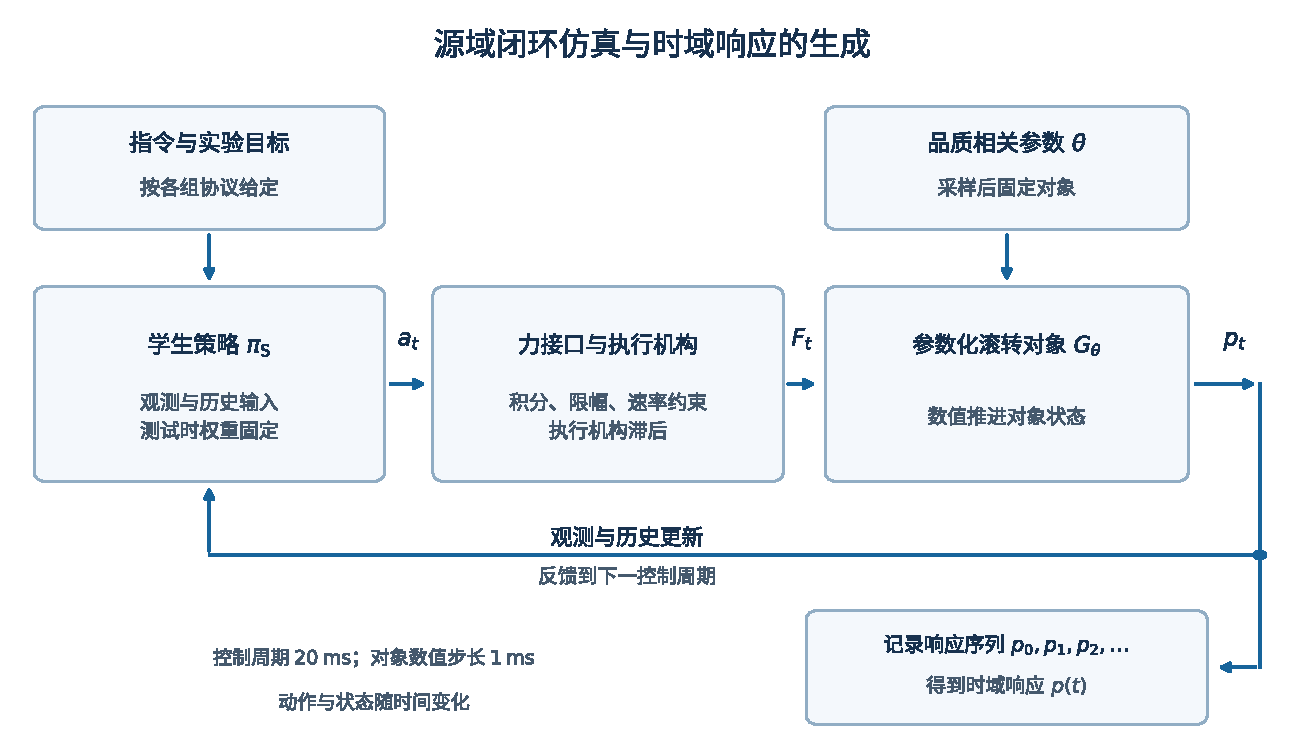
\includegraphics[width=1.00\linewidth,height=.65\textheight,keepaspectratio]{figures/fig01.pdf}
\caption{学生控制器的闭环仿真。品质参数确定对象动态，学生根据观测和历史输出力速率动作，对象响应反馈至下一控制周期。}
\end{figure}
\hypertarget{closed-loop-explanation}{}\label{closed-loop-explanation}
学生每 20 ms 根据当前观测和历史输出动作，仿真器以 1 ms 步长推进对象状态。单条轨迹中，对象参数和策略权重固定，动作、施加力与角速度随反馈更新。按时间记录这些量就得到后文的响应曲线，其中的过冲和振荡取决于对象动态、力接口与控制策略的共同作用。

策略输出归一化力速率动作 \(a_{t}\)。动作经速率约束、积分和限幅形成请求力，再由执行机构动态生成施加力。目标域接口通过力—副翼偏角映射连接 DHC-6 辨识模型，使源域学习与目标域适配采用一致的控制接口。

\hypertarget{observation-inputs}{}\label{observation-inputs}
学生根据任务指令、角速度反馈和控制历史生成动作。输入信号经归一化后组成 176 维观测向量，见表 2。

\hypertarget{observation-table-wrap}{}\label{observation-table-wrap}
\begin{table}[!htbp]\centering
\hypertarget{observation-table}{}\label{observation-table}
\caption{学生控制器的观测组成}
\small\setlength{\tabcolsep}{4pt}\renewcommand{\arraystretch}{1.18}
\begin{tabularx}{\linewidth}{>{\hsize=0.65\hsize\linewidth=\hsize\raggedright\arraybackslash}X>{\hsize=1.95\hsize\linewidth=\hsize\raggedright\arraybackslash}X>{\hsize=0.4\hsize\linewidth=\hsize\raggedright\arraybackslash}X}\toprule
输入部分 & 信号内容 & 维数 \\
\midrule
当前观测 & 指令、目标角速度、实际角速度、跟踪误差、误差积分、实际角速度与目标角速度的导数、请求力、施加力。 & 9 \\
观测历史 & 过去 32 步的指令、目标角速度、实际角速度、跟踪误差和请求力，共 5 个通道。 & 160 \\
动作历史 & 最近 7 步的归一化控制动作。 & 7 \\
\bottomrule\end{tabularx}\end{table}
\begin{equation}\fitmath{\begin{gathered}o_t=\operatorname{Norm}\!\bigl([p_{\mathrm{cmd}},p_{\mathrm{ref}},p,e,\int e\,dt,\dot p,\dot p_{\mathrm{ref}},F_{\mathrm{req}},F_{\mathrm{applied}},h_{t-31:t},a_{t-7:t-1}]\bigr)\in\mathbb R^{176},\\[0.4em]o_t^{\mathrm T}=[o_t,z_t]\in\mathbb R^{188},\qquad o_t^{\mathrm S}=o_t.\end{gathered}}\end{equation}
归一化尺度：指令、参考、响应、误差取 30 deg/s；力取 22 N；角加速度取 5 deg/s\ensuremath{{}^2}；误差积分取 30 deg/s·s。h 为 32\ensuremath{\times}5 历史块，a 为 7 维动作块。

教师使用常规观测和 12 维特权量 \(z_{t}\)，后者包含八个对象参数与四维传递函数实现状态，合计输入维数为 188。学生使用 176 维常规观测，由历史编码分支提取对象动态信息。

\subsection{评价指标与判定门限}
\hypertarget{s23}{}\label{s23}
飞行品质规范用于确定对象模型及分层依据 [1,2,13]。指令跟踪采用目标 RMSE、峰值误差和请求力总变差率评价，项目门限依次为 1.5 deg/s、5 deg/s 和 12 N/s。初始偏差与外力扰动后的恢复另采用 30 s 响应，观察振荡衰减和末段残余。

\hypertarget{pass-rate-definition}{}\label{pass-rate-definition}
同时满足三项门限的测试记为达标，通过率为达标测试数占全部测试数的比例。教师—学生对照与历史表征消融按对象—指令测试组合统计；第 5.3.3 节的 120 对象补充评估按每个对象的归档汇总指标统计。

\begin{equation}\fitmath{\begin{aligned}\operatorname{RMSE}_p&=\sqrt{\frac1M\sum_{t=1}^M(p_{\mathrm{ref},t}-p_t)^2},\\\operatorname{Peak}&=\max_t|p_{\mathrm{ref},t}-p_t|,\\\operatorname{TV}_F&=\frac1T\sum_{t=1}^M|F_{\mathrm{req},t}-F_{\mathrm{req},t-1}|.\end{aligned}}\end{equation}
M 为评价时域内采样点数，T 为评价时长。误差在仿真中按 rad/s 计算、报告时换算为 deg/s；TV\textsubscript{F} 表示请求力总变差率，单位为 N/s。

\hypertarget{distillation-metric}{}\label{distillation-metric}
蒸馏后的相对跟踪精度采用师生闭环跟踪误差比评价。学生与对应教师在相同对象、指令和评价时段下分别运行，对各对象的跟踪 RMSE 比值取中位数：

\hypertarget{distillation-metric-equation}{}\label{distillation-metric-equation}
\begin{equation}\fitmath{R_{\mathrm D}=\operatorname*{median}_{i\in I}\left(\frac{\operatorname{RMSE}_{p,i}^{\mathrm S}}{\operatorname{RMSE}_{p,i}^{\mathrm T}}\right).}\end{equation}
\hypertarget{distillation-metric-definition}{}\label{distillation-metric-definition}
其中，\(I\) 为评价对象集合，上标 \(S\)、\(T\) 分别表示学生与对应对象的教师。\(R_{D}\) 以 1 为教师基准，数值越小表示学生相对教师的跟踪误差越低。蒸馏源对象与对象级留出集分别统计。

\hypertarget{distillation-metric-interpretation}{}\label{distillation-metric-interpretation}
误差比反映对象间的典型相对精度，绝对 RMSE 和门限通过率用于判断实际误差与达标覆盖，时域响应则用于观察瞬态过程和残余振荡。教师误差接近零时，误差比对较小的绝对差异也较敏感，需结合绝对误差解释。

\FloatBarrier
\section{基于飞行品质的飞控大模型构建方法}
\hypertarget{s3}{}\label{s3}
本文以面向品质参数化对象族学习的共享飞控策略为模型主体，统一学生承担策略部署，特权教师库提供逐对象控制经验。图 2 给出对象族、教师、统一学生与目标域模型之间的构建关系。

\begin{figure}[!htbp]\centering
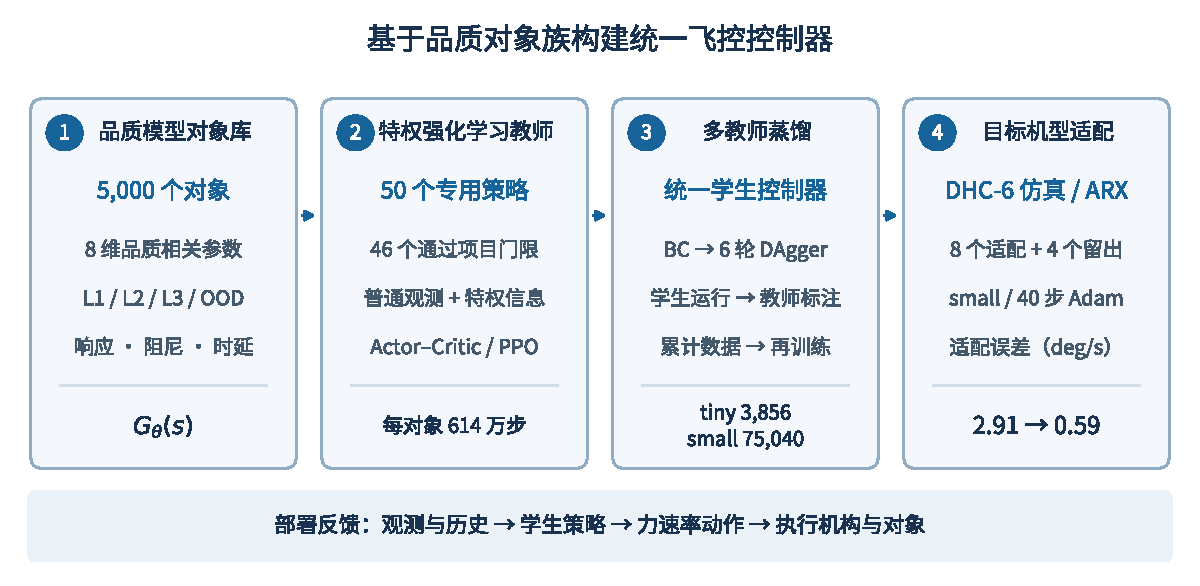
\includegraphics[width=1.00\linewidth,height=.65\textheight,keepaspectratio]{figures/fig02.pdf}
\caption{飞控大模型的构建与验证流程：品质对象族、特权 PPO 教师、多轮蒸馏与目标域适配。tiny 与 small 学生分别含 3,856 和 75,040 个参数；40 次目标域更新及 2.91\ensuremath{\rightarrow}0.59 deg/s 的结果对应 small。}
\end{figure}
\hypertarget{analysis-pipeline-framework}{}\label{analysis-pipeline-framework}
逐对象教师将各自的控制任务转化为动作标签，蒸馏再把这些标签对应的反馈关系合并到共享权重。统一学生在源域对象上以固定权重运行；进入 DHC-6 环节后才利用适配状态更新参数。前一阶段检验跨对象控制，后一阶段考察已有策略在目标模型上的更新效果。

\subsection{品质参数化对象族}
\hypertarget{s31}{}\label{s31}
对象库按 IV 类飞机、A 类飞行阶段的滚转、螺旋、荷兰滚基准和灵敏度相关条件组织候选 [13]。采用九维扰动 Sobol 序列，先确定候选的品质区域，按目标分量设置品质梯度，其余分级分量取基础区域；随后生成模态、时延及灵敏度参数。对每个候选重新计算滚转、螺旋、荷兰滚和灵敏度分量的等级，按其中最差等级分层选入。最终得到 5,000 个对象，L1、L2、L3 各 1,500 个，另有 500 个分布外对象。

\begin{equation}\fitmath{\theta^{(i)}\sim q(\theta\mid c_i),\qquad g_i=\operatorname{Grade}_{\mathrm{src}}(\theta^{(i)},c_i).}\end{equation}
其中，\(\theta^{(i)}\) 为第 \(i\) 个对象的参数向量，\(c_{i}\) 表示候选品质区域，\(q\) 为条件生成与配额筛选形成的分布，\(g_{i}\) 为四项分量判据给出的源域分层标签。参数范围及构造方式见表 3。

\begin{table}[!htbp]\centering
\hypertarget{sampling-protocol-table}{}\label{sampling-protocol-table}
\caption{对象族的候选范围与构造方式}
\small\setlength{\tabcolsep}{4pt}\renewcommand{\arraystretch}{1.18}
\begin{tabularx}{\linewidth}{>{\hsize=0.42\hsize\linewidth=\hsize\raggedright\arraybackslash}X>{\hsize=1.62\hsize\linewidth=\hsize\raggedright\arraybackslash}X>{\hsize=0.96\hsize\linewidth=\hsize\raggedright\arraybackslash}X}\toprule
参数 & 同分布候选的生成与筛选 & 分布外扩展 \\
\midrule
\(L_{F_a}\) & 由 1 s 滚转角灵敏度反标；同分布筛选包络为 \([0.04,\,0.47083875]\) & 将标定后效能超出该包络的候选归入分布外。 \\
\(T_R\) & 按对数尺度映射；基础区间为 \([0.18,\,1.0]\) s，等级扩展上限为 1.4、10 s。 & 慢滚转候选扩展至 \((10,\,15]\) s。 \\
\(\lambda_s\) & 按线性尺度映射；基础区间为 \([-0.15,\,\ln 2/12]\) \(\mathrm{s}^{-1}\)，等级扩展上限为 \(\ln 2/8\)、\(\ln 2/4\)。 & 不稳定根扩展至 \((\ln 2/4,\,0.30]\) \(\mathrm{s}^{-1}\)。 \\
\(\zeta_d\) & 与模态频率联合取值，候选范围为 \([0.005,\,0.70]\)；按阻尼比及阻尼与频率乘积的分级条件设置下限。 & 沿用阻尼构造，允许频率超出常规分级范围。 \\
\(\omega_d\) & 按对数尺度映射；基础区间为 \([1,\,6]\) rad/s；频率项决定二级时取 \([0.4,\,0.99]\) rad/s，三级低阻尼候选取 \([0.4,\,2]\) rad/s。 & 低频候选扩展至 \([0.20,\,0.40)\) rad/s。 \\
\(R_\omega\) & 按对数尺度映射到 \([0.65,\,1.35]\)。 & 现有库的分支映射取值约为 \([0.30,\,0.424]\) 或 \([2.121,\,3.0]\)。 \\
\(R_\zeta\) & 先在线性尺度上选取 \(\zeta_\phi\in[0.1,\,0.7]\)，再令 \(R_\zeta=\zeta_\phi/\zeta_d\)。 & 采用相同的比值构造。 \\
\(\tau_p\) & 按线性尺度映射到 \([0.001,\,0.20]\) s。 & 长时延候选扩展至 \((0.25,\,0.50]\) s。 \\
\bottomrule\end{tabularx}\end{table}
\hypertarget{gain-calibration-protocol}{}\label{gain-calibration-protocol}
操纵效能的标定以 1 N 阶跃作用下的响应为基础：对角速度积分，取 1 s 时刻滚转角的绝对值与输入力幅值之比作为灵敏度。灵敏度目标按对数尺度从 0.85–3.38 deg/N 选取，二级候选扩展至 5.62 deg/N，分布外候选扩展至 8.43 deg/N。每次针对选定的分级分量扩展取值，再重新检查完整参数组合。

\hypertarget{ood-generation-protocol}{}\label{ood-generation-protocol}
分布外划分同时考虑分级边界和参数包络，包括过大的滚转时间常数、不稳定螺旋根、低于 0.4 rad/s 的模态频率、高于 5.62 deg/N 的灵敏度，以及超出效能、零点频率比或时延包络的组合。5,000 个对象按对象编号划为 3,000 个训练候选、450 个验证对象、1,050 个同分布测试对象和 500 个分布外测试对象；教师训练、蒸馏及后续抽样使用这些对象池中的相应子集。

\subsection{特权强化学习教师}
\hypertarget{s32}{}\label{s32}
对选定的 50 个源域对象分别训练 PPO 教师 [3]。逐对象训练将对象动态差异分解为独立控制任务，教师利用已知参数和模型内部状态学习相应反馈策略。Actor 依据式 (2) 的常规观测与特权量输出归一化动作 \(a_{t}\) \ensuremath{\in} [\ensuremath{-}1,1]。在 50 Hz 策略频率下，请求力每步最多变化 1.76 N，并限制于 \ensuremath{\pm}22 N。

\begin{equation}\fitmath{\begin{gathered}F_{\mathrm{req},t+1}=\operatorname{clip}\!\left(F_{\mathrm{req},t}+(88\,\mathrm{N/s})a_t\Delta t,-22\,\mathrm N,22\,\mathrm N\right),\\\Delta t=0.02\,\mathrm s.\end{gathered}}\end{equation}
源域的力接口以 1 kHz 更新，命令力按 88 N/s 跟随请求力，再经时间常数 20 ms 的一阶执行机构模型作用于对象。\ensuremath{\pm}22 N、88 N/s 和 20 ms 共同定义源域实验的操纵权限与执行机构动态，各对象采用相同配置。

教师 Actor 以一维卷积编码历史，并由残差主干产生动作分布，参数量约为 4.26 M。均值头采用无偏置线性层，并对常规观测与内部状态施加奇对称投影，对象参数在镜像变换中保持不变。表 4 列出网络结构和训练设置。

\subsubsection{即时奖励函数}
\hypertarget{s321}{}\label{s321}
即时奖励由跟踪误差、施加力和力速率动作三项组成。令 \(e_{t}\) = \(p_{\mathrm{ref},t}\) \ensuremath{-} \(p_{t}\)，角速度归一化尺度 \(p_{\mathrm{scale}}\) = 30 deg/s，则：

\begin{equation}\fitmath{r_t=-50\left[\left(\frac{e_t}{p_{\mathrm{scale}}}\right)^2\Delta t+0.02\left(\frac{F_{\mathrm{applied},t}}{22\,\mathrm N}\right)^2\Delta t+0.02a_t^2\right].}\end{equation}
误差项驱动策略跟踪目标速率，施加力项约束操纵强度，动作幅值项约束请求力的更新强度。三项共同形成跟踪精度与控制活动之间的优化权衡。

\subsubsection{PPO 优化目标}
\hypertarget{s322}{}\label{s322}
采用广义优势估计（GAE）评价已采样动作的相对收益，时序差分残差与优势递推为：

\begin{equation}\fitmath{\begin{aligned}\delta_t&=r_t+\gamma V_{v_{\mathrm{old}}}(s_{t+1})-V_{v_{\mathrm{old}}}(s_t),\\\widehat A_t&=\delta_t+\gamma\lambda\widehat A_{t+1},\qquad\gamma=0.995,\quad\lambda=0.95.\end{aligned}}\end{equation}
令 \(\rho_{t}\)(w) 为新旧策略对同一已采样动作的概率比，PPO 剪切代理损失为：

\begin{equation}\fitmath{\begin{gathered}\mathcal L_{\mathrm{clip}}(w)=-\mathbb E_t\!\left[\min\!\left(\rho_t\widehat A_t,\operatorname{clip}(\rho_t,1-\epsilon,1+\epsilon)\widehat A_t\right)\right],\\\epsilon=0.2.\end{gathered}}\end{equation}
训练同时优化策略损失、价值估计误差与熵正则项。优势与回报目标由采样时的价值网络计算，并在本轮参数更新中保持固定：

\begin{equation}\fitmath{\begin{aligned}\mathcal L_{\mathrm{total}}&=\mathcal L_{\mathrm{clip}}+0.5\,\mathbb E[(V_v(s_t)-\widehat R_t)^2]-0.001\,\mathcal H(\pi_w),\\\widehat R_t&=\widehat A_t+V_{v_{\mathrm{old}}}(s_t).\end{aligned}}\end{equation}
每个对象训练 30 轮，每轮由 512 个并行环境各运行 400 个策略步，累计约 614 万个状态转移。Actor 与 Critic 使用 Adam，学习率为 3\ensuremath{\times}10\textsuperscript{\ensuremath{-}4}。

\subsubsection{飞行品质、奖励与评价的分工}
\hypertarget{s323}{}\label{s323}
飞行品质参数定义控制对象的动态特征和等级覆盖，奖励函数驱动教师优化跟踪与操纵强度，性能门限则统一评价跟踪误差、峰值和操纵变化。三者分别承担对象组织、策略学习和结果评价的职责，构成从品质描述到控制能力验证的联系。

\begin{table}[!htbp]\centering
\caption{教师网络与训练设置}
\small\setlength{\tabcolsep}{4pt}\renewcommand{\arraystretch}{1.18}
\begin{tabularx}{\linewidth}{>{\hsize=0.35\hsize\linewidth=\hsize\raggedright\arraybackslash}X>{\hsize=1.65\hsize\linewidth=\hsize\raggedright\arraybackslash}X}\toprule
项 & 设置 \\
\midrule
输入 & 本体感受 176 + 特权信息 12 \\
时序前端 & 3 层一维卷积，dilation 1/4/8，感受野 27 步 \\
主干 & 残差 MLP 512 \ensuremath{\times} 8，pre-LN、SiLU、无偏置均值头、奇对称投影 \\
输出 & 归一化增量动作 \ensuremath{\pm}1 \ensuremath{\rightarrow} 请求力每步变化至多 \ensuremath{\pm}1.76 N；请求力限幅 \ensuremath{\pm}22 N \\
算法 & PPO，614 万步/架，\ensuremath{\gamma} 0.995，\ensuremath{\lambda} 0.95，clip 0.2 \\
规模 & 4.26 M 参数，单卡约 9.5 min/架 \\
\bottomrule\end{tabularx}\end{table}
\begin{figure}[!htbp]\centering
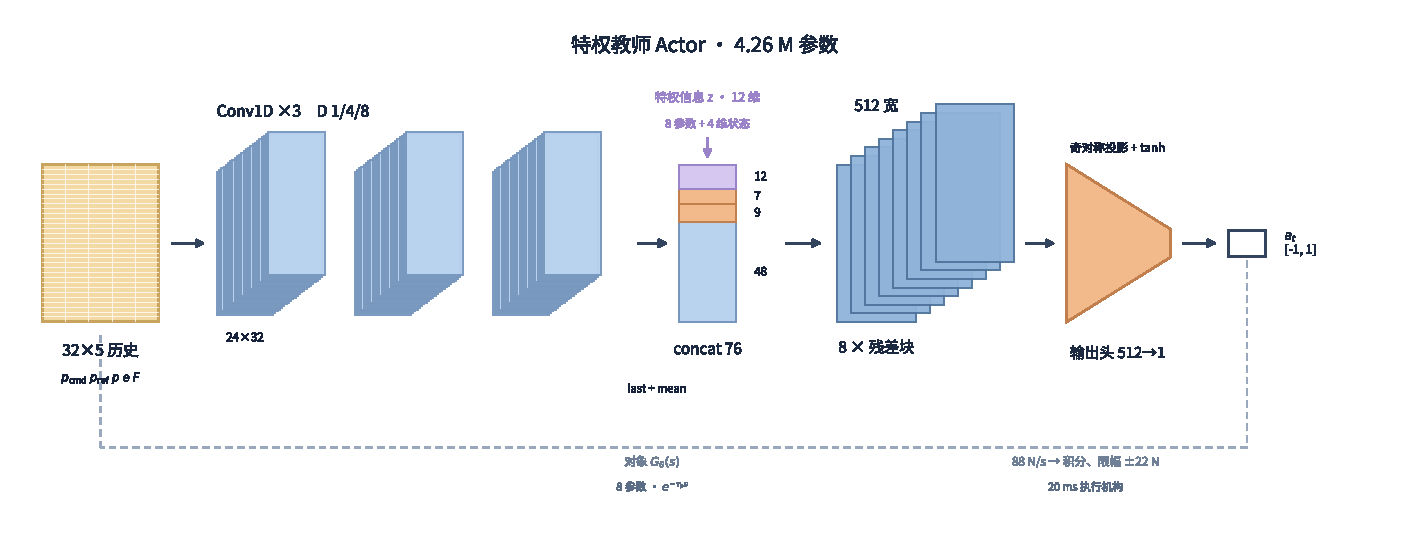
\includegraphics[width=1.00\linewidth,height=.65\textheight,keepaspectratio]{figures/fig03.pdf}
\caption{特权教师 Actor：三层 24 通道卷积形成 48 维历史特征，与 9 维当前量、7 维动作历史和 12 维特权量拼接为 76 维；残差主干含 8 个 512 宽残差块，约 4.26 M 参数。}
\end{figure}
\hypertarget{analysis-teacher-network-tensor}{}\label{analysis-teacher-network-tensor}
教师的 12 维特权量包含对象参数和内部状态，使其能够直接利用当前对象的动态信息。历史分支同时保留过去的输入与响应。两类信息共同用于专用策略训练，其输出动作随后作为学生的监督标签。

\subsection{多教师迭代蒸馏}
\hypertarget{s33}{}\label{s33}
统一学生通过动作模仿汇聚多对象教师的控制经验。主试验学生从 44 个蒸馏源对象的对应教师采集标签，另设 4 个学生对象级留出。初始样本由教师访问闭环状态并标注动作；后续每轮由学生在对象上运行，再由该对象对应的教师提供动作标签 [4]。经过初始行为克隆与 DAgger 迭代，分别得到 3,856 参数的 tiny 学生和 75,040 参数的 small 学生，两者均以常规观测和历史作为部署输入。

\begin{equation}\fitmath{\begin{aligned}D_0&=\{(o_t,\mu_{\mathrm T}(o_t,z_t))\},\\D_{k+1}&=D_k\cup\{(o_t^{\mathrm S,k},\mu_{\mathrm T}(o_t^{\mathrm S,k},z_t))\}.\end{aligned}}\end{equation}
其中，\(\mu_{T}\) 为教师策略，\(z_{t}\) 为对象参数与模型内部状态。第 \(k\) 轮学生产生访问状态后，对应教师利用该状态给出监督动作。学生通过最小化聚合样本上的动作均方误差学习共享策略：

\begin{equation}\fitmath{w_{\mathrm S}^{*}=\operatorname*{arg\,min}_w\frac1{|D_K|}\sum_{(o,u_{\mathrm T})\in D_K}\|\mu_{\mathrm S}(o;w)-u_{\mathrm T}\|^2.}\end{equation}
多轮聚合在学生访问的状态上持续追加教师标签，扩展训练样本的状态覆盖。训练中的动作均方误差约束师生动作差异；蒸馏后的控制能力通过冻结权重的闭环测试评价，指标见第 2.3 节。

\begin{figure}[!htbp]\centering
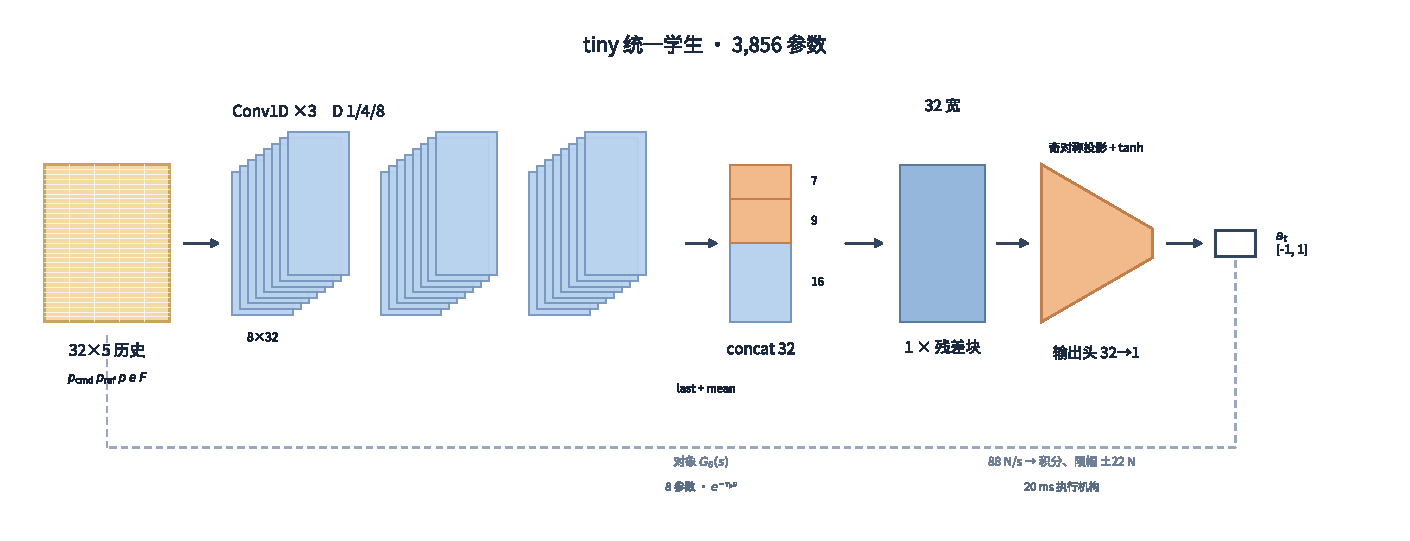
\includegraphics[width=1.00\linewidth,height=.65\textheight,keepaspectratio]{figures/fig04.pdf}
\caption{tiny 学生网络：32\ensuremath{\times}5 历史经时序编码得到 16 维特征，与 9 维当前量和 7 维动作历史拼接为 32 维输入，经一个 32 宽残差块输出动作，共 3,856 个参数。}
\end{figure}
\hypertarget{analysis-student-network-tensor}{}\label{analysis-student-network-tensor}
学生将 160 维历史编码为 16 维特征，再与当前量和动作历史合并后计算控制动作。部署输入中没有独立的对象参数向量或模型内部状态，跨对象响应的差异需要通过反馈历史体现。3,856 个参数对应的是一套共享策略，各对象使用同一组权重。

\subsubsection{历史表征与稀疏编码对照}
\hypertarget{s331}{}\label{s331}
多教师蒸馏同时包含两种变化：将多个对象的控制经验合并到一套权重，并撤去教师使用的对象参数和内部状态。部署学生因而需要利用可观测的输入—响应历史区分对象动态。基线学生将 32\ensuremath{\times}5 历史送入随控制任务联合训练的时序编码器，得到 16 维历史特征。历史中的对象信息能否被有效利用，是统一控制器输入设计需要检验的问题。

为检验显式表征学习能否改善对象动态信息的提取，设置 PCA、稠密自编码器和稀疏自编码器（SAE）前端对照。SAE 检验少数活跃特征能否集中保留对象动态线索，稠密编码用于比较稀疏约束的影响。SAE 采用 160\ensuremath{\rightarrow}64\ensuremath{\rightarrow}16 编码器和对称解码器，以 L1 或 top-k 约束限制潜码中的活跃分量。替换分支用冻结前端输出的 16 维特征替代基线时序特征；辅助分支在保留基线特征时再附加 SAE 潜码。各替换前端的历史特征维度均为 16，用于比较不同表征学习方式。

评价分为信息读出和闭环控制两步：以对象输入运输时延 \(\tau_{p}\) 为标签，检验因果历史中能否读出对象动态线索；再将相同表征接入策略，比较跟踪与恢复过程。探针和控制结果共同用于判断输入设计。该消融在既有 tiny 学生上进行，动作标签由该学生产生；原始历史与辅助输入分支继承其权重，替换分支训练新的策略头。完整网络和训练设置见\hyperlink{s611}{附录 A.1}。

\subsection{目标域小样本适配}
\hypertarget{s34}{}\label{s34}
目标域采用 12 个 DHC-6 仿真配平状态的 72 条、50 Hz 输入输出记录。通过扫频激励辨识各状态的 ARX 模型，阶次范围为 na = 4–5、nb = 3–4、nk = 1，拟合 VAF 为 98.0\%–98.7\%。目标域辨识模型以副翼偏角为输入。控制器动作经积分与限幅形成力信号，再按 \(\delta_{a}\) = \ensuremath{-}(10°/22 N)\(F\) 转换为副翼输入，对应本组实验的 \ensuremath{\pm}10° 幅值和 40°/s 速率范围，辨识模型的滚转角速度反馈至策略。

采用 small 学生进行目标域更新，优化其全部 75,040 个参数。8 个配平状态提供适配样本，另外 4 个状态用于更新后的留出评价。优化执行 40 次 Adam 更新，学习率为 3\ensuremath{\times}10\textsuperscript{\ensuremath{-}5}；损失统计响应开始 2 s 后的跟踪平方误差。评价使用确定性策略、15 deg/s 正阶跃及 8 s 时域。

\begin{equation}\fitmath{\begin{aligned}e_t(W)&=p_{\mathrm{ref},t}-p_t(W;\widehat G_{\mathrm{ARX}}),\\\mathcal L_{\mathrm{DHC6}}(W)&=\frac1{N_{t\ge2\,\mathrm s}}\sum_{t\ge2\,\mathrm s}e_t(W)^2,\\W_{k+1}&=\operatorname{AdamUpdate}(W_k,\nabla_W\mathcal L_{\mathrm{DHC6}};\eta=3\times10^{-5}).\end{aligned}}\end{equation}
式中，\(W\) 为学生参数，Ĝ\textsubscript{ARX} 为适配状态的辨识模型。适配组用于参数更新，留出组用于观察更新所得控制知识的跨状态复用。

\FloatBarrier
\section{实验设置}
\hypertarget{s4}{}\label{s4}
实验围绕滚转通道的构建路线展开：主试验检验教师学习与学生蒸馏，配对实验检验专用教师迁移与统一学生的多对象控制，表征对照分析历史输入设计，DHC-6 仿真检验目标域适配。各组的对象集、控制器与评价协议见表 5。

\subsection{对象划分与评价协议}
\hypertarget{experiment-data-protocol}{}\label{experiment-data-protocol}
\begin{table}[!htbp]\centering
\caption{数据划分与评估协议}
\small\setlength{\tabcolsep}{4pt}\renewcommand{\arraystretch}{1.18}
\begin{tabularx}{\linewidth}{>{\hsize=1\hsize\linewidth=\hsize\raggedright\arraybackslash}X>{\hsize=1\hsize\linewidth=\hsize\raggedright\arraybackslash}X>{\hsize=1\hsize\linewidth=\hsize\raggedright\arraybackslash}X>{\hsize=1\hsize\linewidth=\hsize\raggedright\arraybackslash}X}\toprule
阶段 & 对象 / 数据 & 训练与留出 & 被评内容 \\
\midrule
对象库 & 5,000 个参数化滚转模型 & 4,500 个训练/同分布池；500 个分布外 & 参数与品质等级覆盖 \\
PPO 教师 & 50 个源域对象 & 已有 46 个通过项目门限 & 确定性闭环跟踪与操纵 \\
学生 & 48 个源域对象 & 44 个蒸馏；4 个留出，等级各 16 个 & tiny / small 跨对象性能 \\
DHC-6 微调 & 12 个仿真配平状态、72 条记录 & 8 个适配；4 个留出 & small 学生、单随机种子 \\
库规模抽样 & 4,500 个非 OOD 对象池 & 每级随机抽 40 个，共 120 个 & tiny 学生，随机种子 20261023 \\
幅值 / OOD & 300 个同分布对象、500 个 OOD 对象 & 14 条指令/对象；每指令重复 2 次 & tiny 学生固定权重，11,200 个对象—指令组合 \\
\bottomrule\end{tabularx}\end{table}
主试验学生在 48 个对象上采用 30 条加权指令和每对象 64 条并行确定性轨迹评价。幅值扫描包含 300 个同分布对象、500 个分布外对象及 14 条输入配置，每个对象—指令组合重复两次。12 对象配对组包含三组训练重复；DHC-6 以配平状态为适配和留出单元，在固定阶跃及单一策略种子下评价。各组分别按其对象和测试单元统计。

\FloatBarrier
\section{滚转通道验证}
\hypertarget{s5}{}\label{s5}
\subsection{品质对象族的动态覆盖}
\hypertarget{s51}{}\label{s51}
5,000 个对象在参数空间中的分布如图 5 所示，其中三个品质等级各 1,500 个，分布外对象为 500 个。各参数的边际分布见附录 B.1。

\begin{figure}[!htbp]\centering
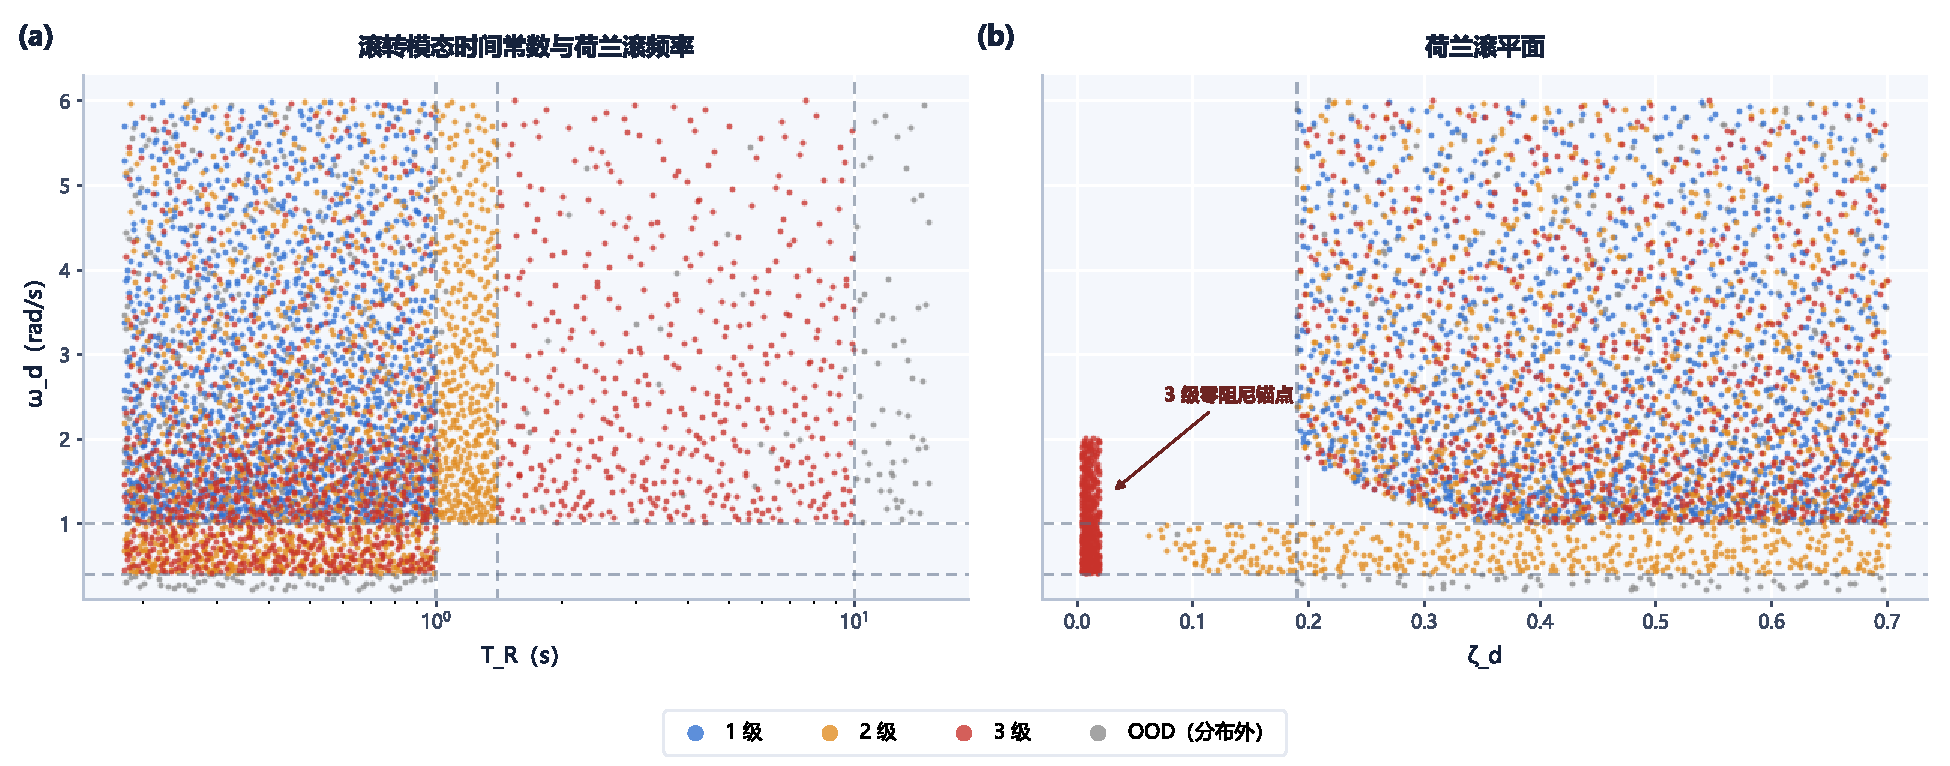
\includegraphics[width=1.00\linewidth,height=.65\textheight,keepaspectratio]{figures/fig05.pdf}
\caption{5,000 个对象的参数空间投影。颜色区分三个品质等级与分布外对象，虚线标出所选分级边界。}
\end{figure}
\hypertarget{analysis-sampling-scatter}{}\label{analysis-sampling-scatter}
时间常数—频率平面覆盖了快、慢滚转及低频模态，阻尼—频率平面则显示不同的振荡衰减条件。各等级在二维投影中仍有重叠，因为分级还涉及螺旋模态和灵敏度。部分分布外对象也落在图示坐标的常规范围内，它们的越界发生在其他参数或参数组合上。

\subsection{专用教师的控制能力}
\hypertarget{s52}{}\label{s52}
主试验选取 50 个源域对象开展逐对象教师训练，已有 46 个教师达到统一性能门限。图 6 给出三个品质等级代表对象的阶跃与多正弦响应，训练诊断和对象参数与误差的关系见附录 B.1。

\begin{figure}[!htbp]\centering
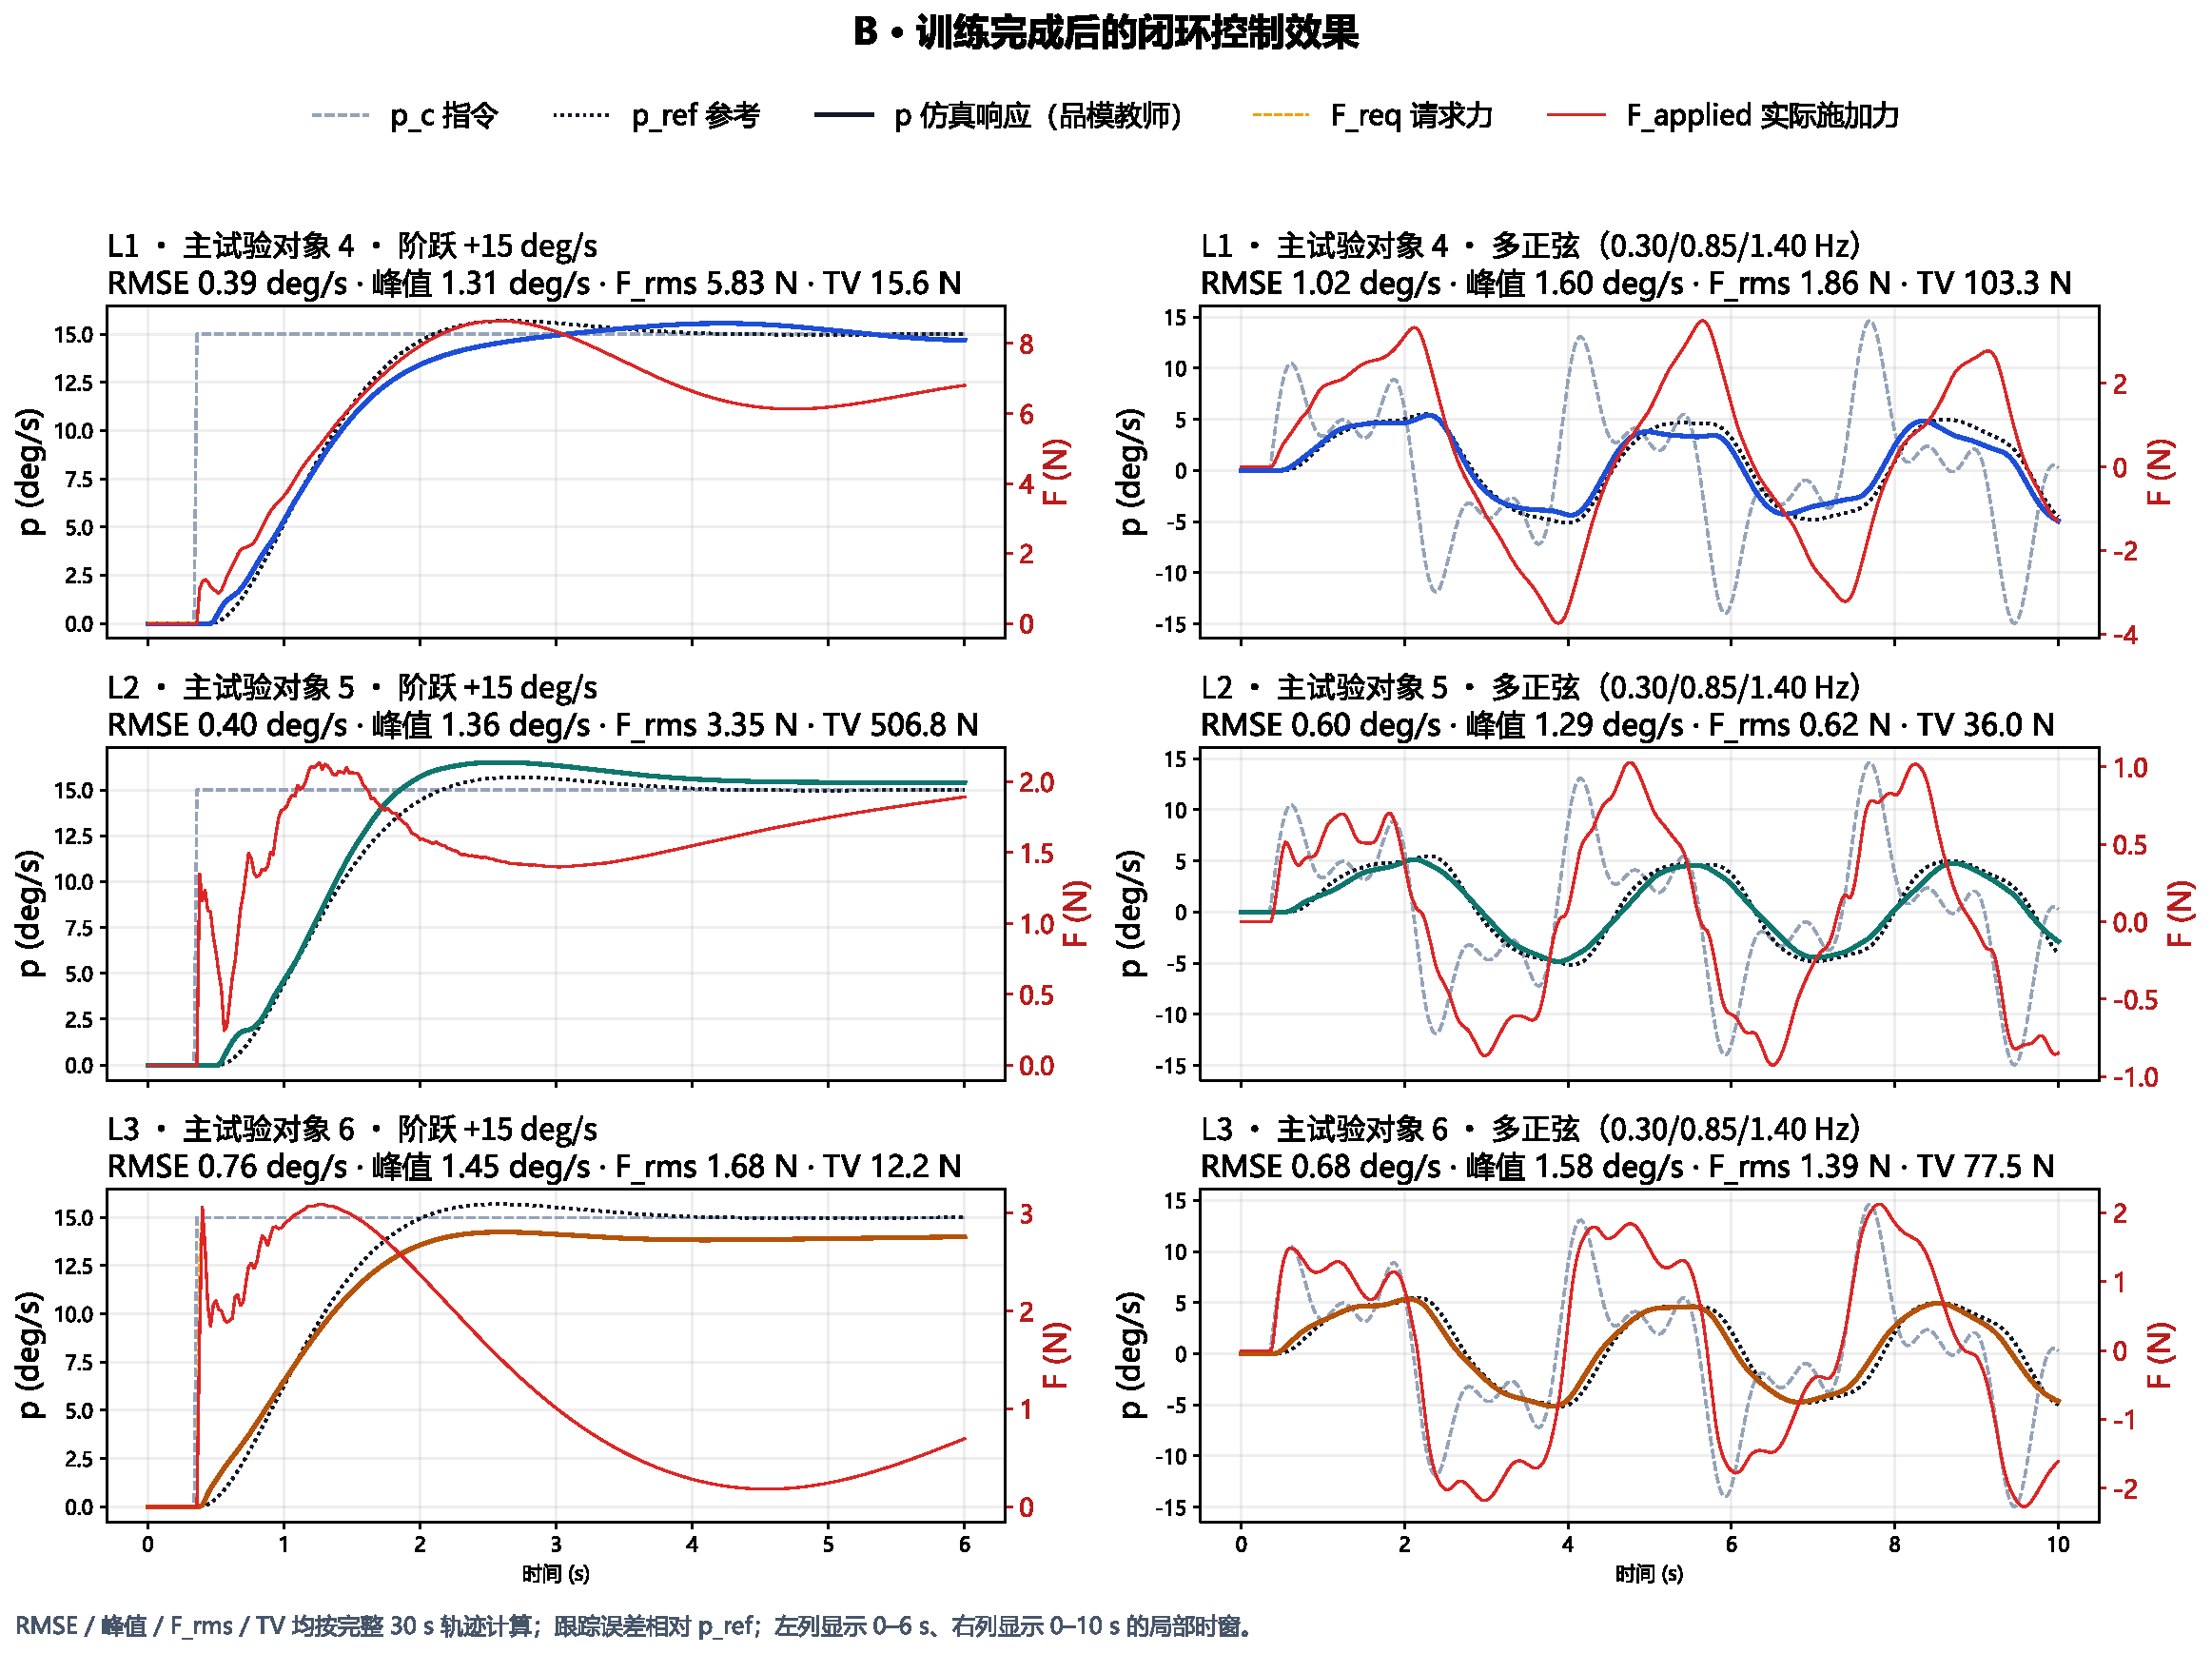
\includegraphics[width=1.00\linewidth,height=.65\textheight,keepaspectratio]{figures/fig06.pdf}
\caption{教师训练完成后的源域闭环效果：不同品质等级的阶跃与多正弦响应。}
\end{figure}
\hypertarget{analysis-teacher-closed-loop}{}\label{analysis-teacher-closed-loop}
三个代表对象的阶跃跟踪 RMSE 为 0.39–0.76 deg/s，多正弦下为 0.60–1.02 deg/s。跟踪误差接近时，操纵变化仍有明显差别：二级阶跃样例的请求力持续调整，完整 30 s 的总变差达到 506.8 N。图内的 TV 是总变差，项目指标则使用除以时长后的变化率；两者分别描述整段操纵累积和单位时间内的操纵活动。

\subsection{统一策略的知识汇聚与跨对象控制}
\hypertarget{s53}{}\label{s53}
\hypertarget{distillation-results}{}\label{distillation-results}
学生先通过行为克隆学习教师动作，再进行五轮 DAgger 数据聚合。图 7 将行为克隆记为第 0 轮，随后记录第 1–5 轮聚合后的闭环结果。

\begin{figure}[!htbp]\centering
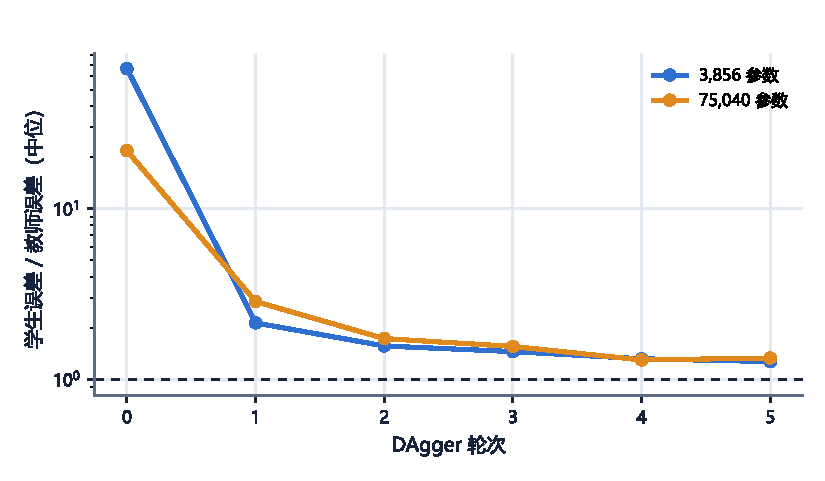
\includegraphics[width=0.60\linewidth,height=.65\textheight,keepaspectratio]{figures/fig07.pdf}
\caption{DAgger 轮次与师生闭环跟踪误差比。第 0 轮为行为克隆，随后在学生访问状态上追加教师标签。}
\end{figure}
\hypertarget{analysis-student-dagger}{}\label{analysis-student-dagger}
追加学生访问状态上的教师标签后，误差比在前几轮下降较快，后期曲线趋于平缓。tiny 与 small 的源对象误差比分别达到 1.28、1.34；在 44 个源对象中分别有 37、38 个达标。留出对象的误差比为 1.68、1.41，两者均通过 3/4。参数规模、控制覆盖与相对精度的完整统计见表 6。

\hypertarget{distillation-results-table-wrap}{}\label{distillation-results-table-wrap}
\begin{table}[!htbp]\centering
\hypertarget{distillation-results-table}{}\label{distillation-results-table}
\caption{两种规模学生的源域结果}
\small\setlength{\tabcolsep}{4pt}\renewcommand{\arraystretch}{1.18}
\begin{tabularx}{\linewidth}{>{\hsize=1\hsize\linewidth=\hsize\raggedright\arraybackslash}X>{\hsize=1\hsize\linewidth=\hsize\raggedright\arraybackslash}X>{\hsize=1\hsize\linewidth=\hsize\raggedright\arraybackslash}X>{\hsize=1\hsize\linewidth=\hsize\raggedright\arraybackslash}X>{\hsize=1\hsize\linewidth=\hsize\raggedright\arraybackslash}X>{\hsize=1\hsize\linewidth=\hsize\raggedright\arraybackslash}X}\toprule
学生 & 参数量 & 源对象通过 & 留出对象通过 & 源对象误差比 & 留出对象误差比 \\
\midrule
tiny & 3,856 & 37/44 & 3/4 & 1.28\ensuremath{\times} & 1.68\ensuremath{\times} \\
small & 75,040 & 38/44 & 3/4 & 1.34\ensuremath{\times} & 1.41\ensuremath{\times} \\
\bottomrule\end{tabularx}\end{table}
\subsubsection{代表性闭环响应}
\hypertarget{s531}{}\label{s531}
图 8 比较主试验对象 7 上教师与学生在相同指令下的响应。误差标注采用 2 s 后的评价段。

\begin{figure}[!htbp]\centering
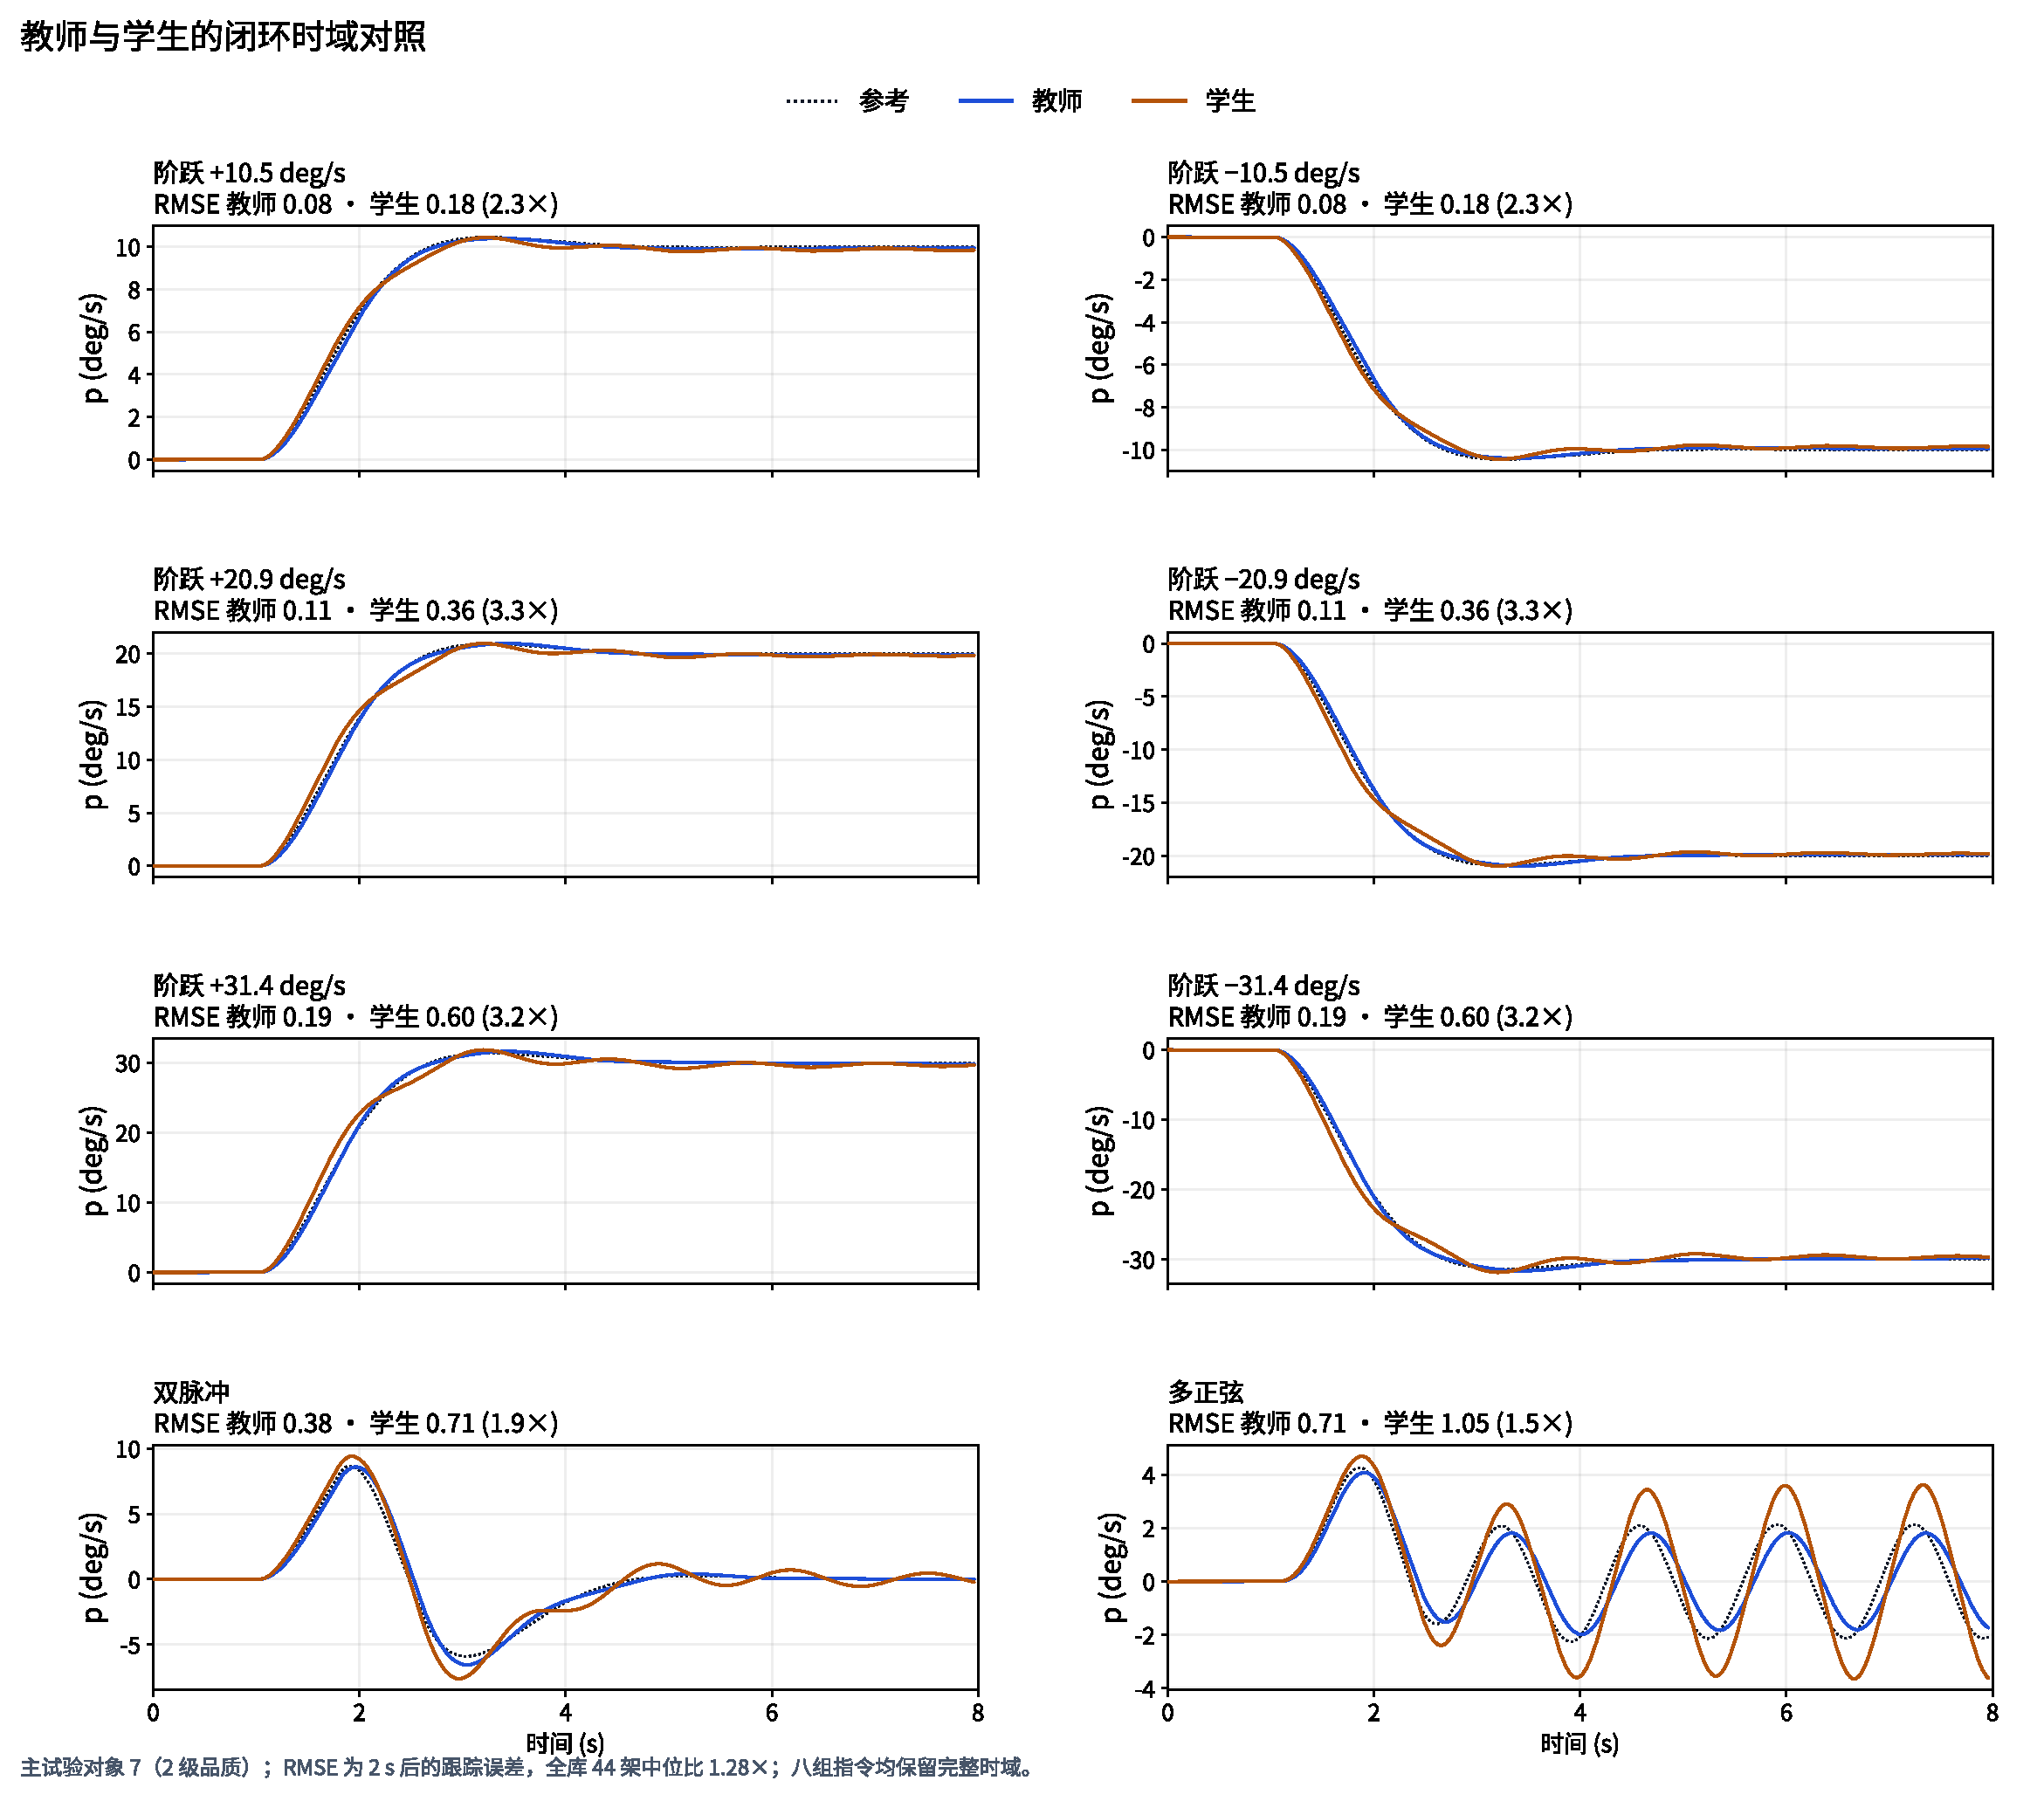
\includegraphics[width=1.00\linewidth,height=.65\textheight,keepaspectratio]{figures/fig08.pdf}
\caption{教师与统一学生在主试验对象 7 上的同指令时域对照。黑色点线为目标，蓝线为教师，橙线为学生；标题报告 2 s 后的跟踪 RMSE 及其比值。}
\end{figure}
\hypertarget{analysis-teacher-student-compare}{}\label{analysis-teacher-student-compare}
正、负阶跃中，师生的主要上升过程接近，学生在 2 s 后的跟踪 RMSE 为教师的 2.3–3.3 倍。双脉冲与多正弦的比值为 1.5–1.9。逐指令响应给出瞬态与稳态行为，对象级中位统计则汇总多对象上的相对跟踪精度。

\subsubsection{跨对象闭环控制性能评估}
\hypertarget{s532}{}\label{s532}
\hypertarget{results-cross-object-details}{}\label{results-cross-object-details}
采用 12 对象配对组比较专用教师与统一学生，每个品质等级含 4 个对象，共三次训练重复；12 个对象均参与相应学生的蒸馏。每个教师依次控制全部对象，学生控制相同对象；每个控制器在每个对象上测试 18 条指令，时域为 8 s。跨对象使用的教师读取当前被控对象的参数与状态，学生依靠常规观测和历史；所有权重固定。

在有限轨迹上，统一学生的跟踪 RMSE 中位数为 0.96 deg/s，自身教师为 0.75 deg/s，教师跨对象使用时为 3.28 deg/s。统一学生以一组共享权重，在多个源对象上保持了与专用教师相近的跟踪误差量级；相较直接跨对象使用专用教师，共享策略获得了更低的跟踪误差。

图 9 在同一被控对象及相同指令、初始偏差和外力扰动下，对照自身教师、跨对象教师与统一学生的跟踪和恢复过程。指令跟踪采用 8 s 时域，初始偏差与扰动恢复采用 30 s 时域。样例按训练阶段的独立验证记录选取。

\begin{figure}[!htbp]\centering
\hypertarget{cross-object-time-response}{}\label{cross-object-time-response}
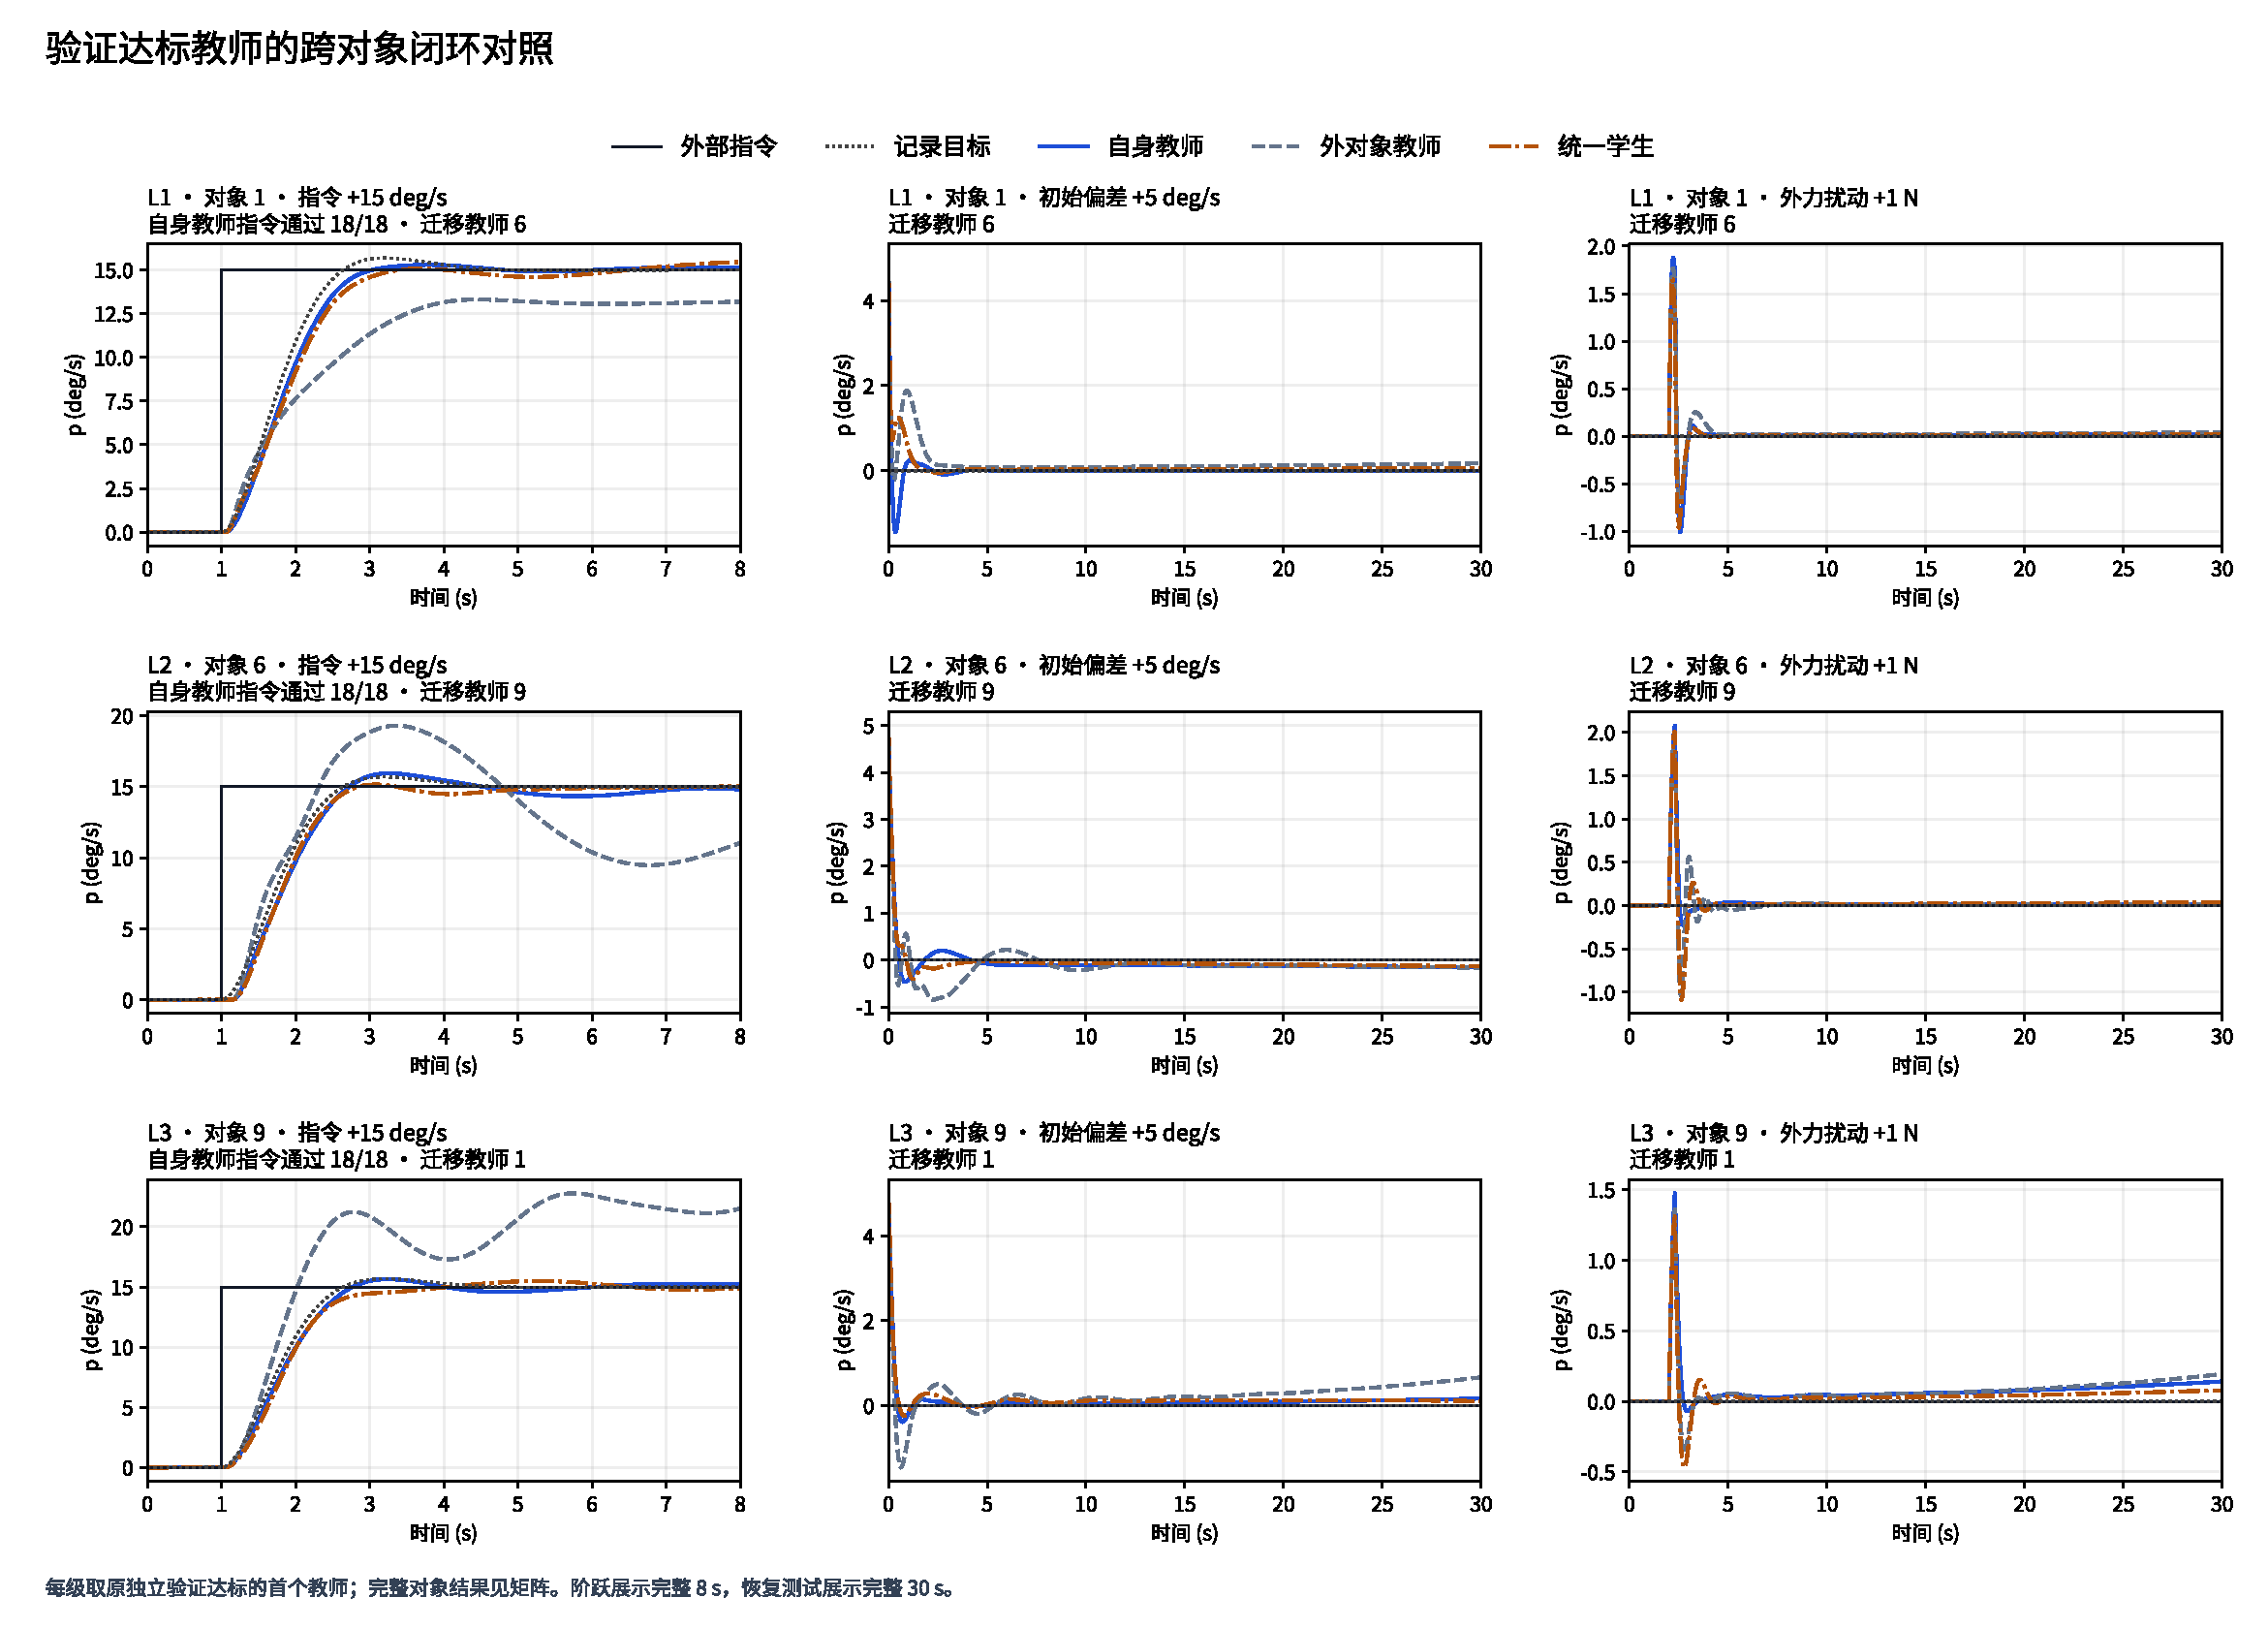
\includegraphics[width=1.00\linewidth,height=.65\textheight,keepaspectratio]{figures/fig09.pdf}
\caption{验证达标教师与统一学生的闭环对照。三行受控对象为 1、6、9，迁移教师为 6、9、1；三列依次展示指令跟踪、初始偏差恢复和外力扰动抑制。黑色实线为外部指令，灰色点线为记录目标。}
\end{figure}
\hypertarget{analysis-cross-object-responses}{}\label{analysis-cross-object-responses}
对象 6、9 上，跨对象教师的阶跃响应出现较大过冲和摆动，统一学生与自身教师的响应更接近。初始偏差和外力扰动测试中，学生的后段残差也较小。对象 9 在 30 s 内仍可见残余偏差，恢复阶段的残余响应需与整段跟踪误差同时评价。

\begin{figure}[!htbp]\centering
\hypertarget{cross-object-matrix}{}\label{cross-object-matrix}
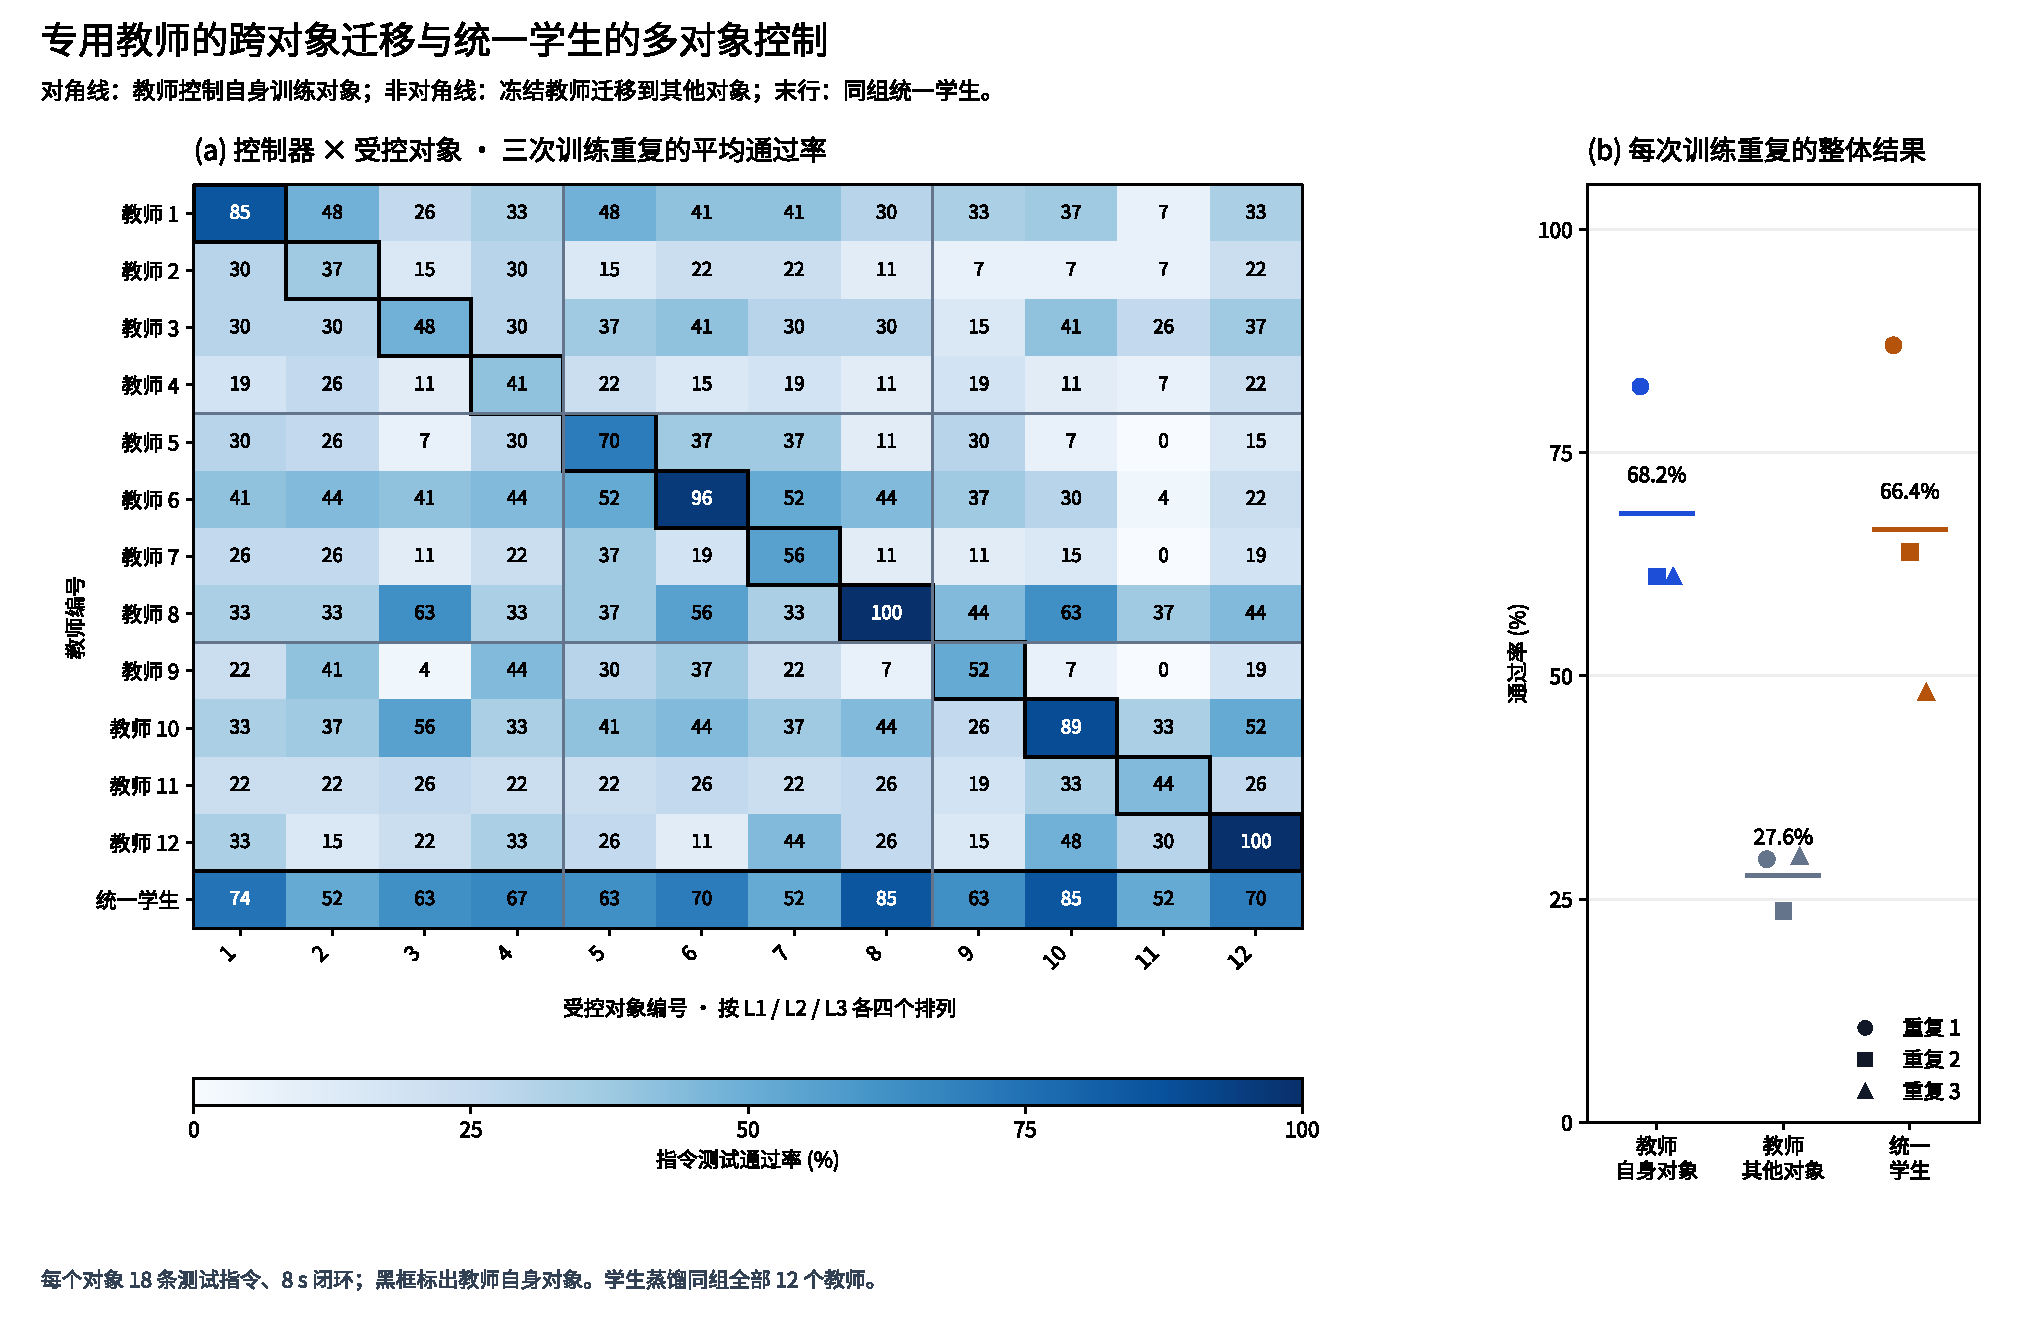
\includegraphics[width=1.00\linewidth,height=.65\textheight,keepaspectratio]{figures/fig10.pdf}
\caption{专用教师跨对象控制与统一学生的对象覆盖。对角线为自身教师，非对角线为跨对象教师，末行为学生；每格汇总三次训练重复。右侧点为各次重复，横线为平均值。}
\end{figure}
\hypertarget{analysis-cross-object-matrix}{}\label{analysis-cross-object-matrix}
教师 1 在自身对象 1 上通过 46/54 条测试，在对象 6 上为 22/54，显示同一专用策略换对象后的差异。学生末行给出一套共享权重在全部 12 个源对象上的结果。三次训练重复的学生整体通过率为 87.0\%、63.9\%、48.1\%，其多对象控制表现也随训练重复变化；完整汇总见下表。

\begin{table}[!htbp]\centering
\hypertarget{cross-object-results}{}\label{cross-object-results}
\caption{配对教师—学生的闭环测试汇总。通过率按全部测试组合统计，RMSE 中位数按有限轨迹统计。}
\small\setlength{\tabcolsep}{4pt}\renewcommand{\arraystretch}{1.18}
\begin{tabularx}{\linewidth}{>{\hsize=1\hsize\linewidth=\hsize\raggedright\arraybackslash}X>{\hsize=1\hsize\linewidth=\hsize\raggedright\arraybackslash}X>{\hsize=1\hsize\linewidth=\hsize\raggedright\arraybackslash}X>{\hsize=1\hsize\linewidth=\hsize\raggedright\arraybackslash}X>{\hsize=1\hsize\linewidth=\hsize\raggedright\arraybackslash}X}\toprule
控制方式 & 通过 / 测试组合 & 通过率 & RMSE 中位 (deg/s) & 超限或非有限终止 \\
\midrule
教师控制自身训练对象 & 442/648 & 68.2\% & 0.75 & 0 \\
教师控制其他对象 & 1970/7128 & 27.6\% & 3.28 & 12 \\
统一学生控制同组对象 & 430/648 & 66.4\% & 0.96 & 0 \\
\bottomrule\end{tabularx}\end{table}
12 对象配对组包含三次训练重复，每次为 12 个专用教师及其统一学生。自身教师和学生各有 648 个对象—指令组合，跨对象教师有 7,128 个组合。响应非有限或角速度绝对值超过 300 deg/s 时记为失败；通过率按全部组合、RMSE 中位数按有限轨迹计算。

三组重复中，学生通过率分别为 87.0\%、63.9\%、48.1\%，自身教师分别为 82.4\%、61.1\%、61.1\%。时域样例按训练阶段独立验证记录选择：第一组 8 个教师达标，每个品质等级依原对象顺序取首个，得到对象 1、6、9，跨对象教师为 6、9、1。选样及验证记录见时域对照协议，完整诊断响应见闭环诊断图。

补充数据：逐控制器—对象数值；编号对照；重复 1 矩阵、重复 2 矩阵、重复 3 矩阵。

\subsubsection{对象覆盖与分布外控制性能}
\hypertarget{s533}{}\label{s533}
采用 300 个同分布对象和 500 个分布外对象评价统一学生的对象覆盖，前者从主试验 48 个评估对象之外抽取。学生权重保持固定，每个对象测试 14 条输入配置，各重复两次，共 22,400 条轨迹，记录跟踪误差、峰值误差与操纵变化。

同分布对象上，\ensuremath{\pm}1 deg/s 和 \ensuremath{\pm}31 deg/s 阶跃的跟踪 RMSE 中位数分别为 0.11、1.13 deg/s；分布外对象上相应为 0.21、2.93 deg/s。这组结果给出同一策略在不同对象分布及指令幅值下的跟踪误差水平。补充控制器对照见\hyperlink{results-pid-comparison}{附录 B.3}。

\hypertarget{s61}{}\label{s61}
按对象级汇总指标评价时，主试验 tiny 学生在 120 个新增同分布对象上通过 94/120（78.3\%），三个等级分别通过 34/40、30/40、30/40，RMSE 中位数为 0.64 deg/s，90 百分位为 2.24 deg/s。这些对象从 4,500 个同分布对象池按每级 40 个抽取，与主试验 48 个评估对象不重叠。

在新增对象中，RMSE 与滚转操纵效能的相关系数为 \ensuremath{-}0.47；滚转时间常数 \(T_{R}\) > 6 s 的 4 个对象中有 1 个通过。对象参数与性能的对应关系为下一阶段扩大训练覆盖提供了具体方向。

\subsubsection{历史表征对照}
\hypertarget{s535}{}\label{s535}
统一学生利用输入—响应历史获取对象动态线索。按第 3.3.1 节的输入设计与训练配置，保留基线时序编码的学生及 SAE 辅助输入方案在长延迟层均达到 90.0\% 通过率，PCA-16、稠密 AE-16、Top-k SAE-16 替换方案分别为 51.6\%、63.7\%、71.9\%。本实现据此采用与控制任务联合学习的时序编码，将历史映射为 16 维特征参与决策。完整闭环对照见\hyperlink{s613}{附录 A.3}，信息读出与长时动态分析见\hyperlink{appendix-history}{附录 A}。

\subsection{DHC-6 目标域适配}
\hypertarget{s54}{}\label{s54}
在 DHC-6 ARX 目标模型上，small 学生经 40 次参数更新，8 个适配状态的 RMSE 中位数由 2.913 降至 0.595 deg/s，4 个留出状态由 2.662 降至 2.148 deg/s，分别降低 79.6\% 和 19.3\%。所有状态均采用 15 deg/s 阶跃和 8 s 评价时域。

\begin{figure}[!htbp]\centering
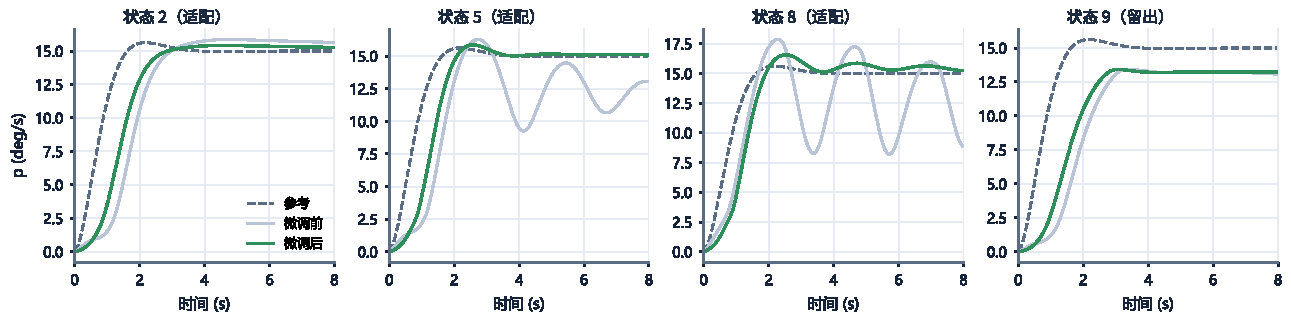
\includegraphics[width=1.00\linewidth,height=.65\textheight,keepaspectratio]{figures/fig11.pdf}
\caption{代表性 DHC-6 仿真状态的微调前后闭环响应。适配状态微调后贴合参考；留出状态保持原策略的响应形态。}
\end{figure}
\hypertarget{analysis-dhc6-states}{}\label{analysis-dhc6-states}
状态 5、8 在微调前有明显摆动，微调后振荡减弱，响应更接近目标；状态 2 的上升段也有所改善。留出的状态 9 在微调前后都低于最终目标速率。各配平状态上的更新效果通过瞬态形态和稳态误差共同描述。逐状态误差及两档模型的对照见附录 B.2。

\FloatBarrier
\section{讨论}
\hypertarget{s6}{}\label{s6}
多教师蒸馏将逐对象控制经验汇入共享策略。12 对象配对组中，统一学生的跟踪 RMSE 中位数为 0.96 deg/s，自身教师为 0.75 deg/s，跨对象教师为 3.28 deg/s。这组对照显示，知识汇聚使一套权重能够复用多个对象的反馈经验；专用教师读取新对象参数后的直接复用具有不同的控制表现。

学生的规模与精度呈现不同变化：small 的留出对象误差比较低，源对象上则略高于 tiny。历史表征对照也显示，较高的参数读出分数不必然对应更好的控制结果。网络规模和输入编码应结合实际闭环误差、操纵变化与恢复动态选择。

DHC-6 更新主要改善了适配状态的跟踪与振荡，留出状态的整体改善幅度较小，且不同状态之间存在差异。后续扩展需围绕目标动态的覆盖，以及执行机构特性和多轴耦合条件下的闭环表现展开。

\FloatBarrier
\section{结论}
\hypertarget{s7}{}\label{s7}
本文提出基于飞行品质的飞控大模型构建路线，并以滚转通道完成从对象组织、特权教师学习、多轮蒸馏到目标域适配的验证。飞行品质参数将对象差异组织为可学习任务，教师控制经验经 DAgger 汇聚为统一策略，实现了控制知识的离线积累与共享。

统一学生以 3,856 个参数保留多对象控制能力，在 44 个蒸馏源对象上的 RMSE 中位比为 1.28。在 500 个分布外对象的 \ensuremath{\pm}1 deg/s 测试中，通过率达到 86.8\%。历史表征对照支持使用任务驱动的时序编码，形成从观测历史到统一控制动作的部署形式。

DHC-6 仿真适配进一步展示了共享策略的更新能力：small 学生经 40 次更新，将适配状态 RMSE 中位数降至 0.59 deg/s，留出状态降至 2.15 deg/s。上述证据共同支撑了基于飞行品质组织控制知识、通过教师—学生学习形成统一飞控策略的技术路线。

\FloatBarrier
\begin{thebibliography}{99}
\bibitem{ref1} GJB 185-1986. 有人驾驶飞机（固定翼）飞行品质[S]. 北京: 国防科学技术工业委员会, 1986.
\bibitem{ref2} MIL-STD-1797A. Flying qualities of piloted aircraft[S]. Washington: Department of Defense, 1990.
\bibitem{ref3} J. Schulman, F. Wolski, P. Dhariwal, et al. Proximal policy optimization algorithms[J]. arXiv:1707.06347, 2017.
\bibitem{ref4} S. Ross, G. Gordon, D. Bagnell. A reduction of imitation learning and structured prediction to no-regret online learning[C]. AISTATS, 2011.
\bibitem{ref5} V. Vapnik, A. Vashist. A new learning paradigm: learning using privileged information[J]. Neural Networks, 2009, 22(5-6): 544-557.
\bibitem{ref6} L. Pinto, M. Andrychowicz, P. Welinder, et al. Asymmetric actor critic for image-based robot learning[C]. Robotics: Science and Systems, 2018. \href{https://www.roboticsproceedings.org/rss14/p08.html}{原文}
\bibitem{ref7} J. Lee, J. Hwangbo, L. Wellhausen, et al. Learning quadrupedal locomotion over challenging terrain[J]. Science Robotics, 2020, 5(47).
\bibitem{ref8} T. Miki, J. Lee, J. Hwangbo, et al. Learning robust perceptive locomotion for quadrupedal robots in the wild[J]. Science Robotics, 2022, 7(62).
\bibitem{ref9} A. Kumar, Z. Fu, D. Pathak, et al. RMA: Rapid motor adaptation for legged robots[C]. Robotics: Science and Systems, 2021.
\bibitem{ref10} M. O'Connell, G. Shi, X. Shi, et al. Neural-Fly enables rapid learning for agile flight in strong winds[J]. Science Robotics, 2022, 7(66): eabm6597. \href{https://doi.org/10.1126/scirobotics.abm6597}{原文}
\bibitem{ref11} E. Kaufmann, L. Bauersfeld, A. Loquercio, et al. Champion-level drone racing using deep reinforcement learning[J]. Nature, 2023, 620: 982-987.
\bibitem{ref12} J. Eschmann, D. Albani, G. Loianno. Learning to fly in seconds[J]. IEEE Robotics and Automation Letters, 2024.
\bibitem{ref13} GJB 2874—1997. 电传操纵系统飞机的飞行品质[S]. 1997.
\end{thebibliography}
\FloatBarrier
\appendix
\ctexset{section/name={附录~,},section/number=\Alph{section}}
\section{历史表征对照与闭环动态诊断}
\hypertarget{appendix-history}{}\label{appendix-history}
本附录给出第 3.3.1 节与第 5.3.4 节历史表征消融的完整设置、探针结果和闭环诊断，便于核对输入设计的依据。

\subsection{历史表征的数据与训练设置}
\hypertarget{s611}{}\label{s611}
基线的时序编码器与控制策略联合训练，将 160 维历史映射为 16 维特征，再与 9 维当前量、7 维旧动作拼接。替换前端也输出 16 维并冻结，只训练后续策略头；辅助前端则在基线特征之外增加 16 维潜码。该对照比较的是表征学习方式及其训练配置。

从第 3.1 节对象库的 训练集、验证集和留出测试集 三个互不重叠的划分中，按 \(\tau_{p}\) 的短、中、长三层分别抽取 100、30、40 个，共 510 个。每个对象运行 8 条指令，包括 +1、+2、+5、+10、+21、+31 deg/s 阶跃、双脉冲和多正弦；由既有 tiny 学生闭环驱动，记录 32\ensuremath{\times}5 历史、当前量、旧动作和动作，共 489,600 个窗口。留出集为 120 个、960 个对象—指令 episode。训练、验证和测试按对象划分。

图 12 给出两种使用历史的方式：主线学生保留原始历史；表征分支将 160 维展平历史压缩为 16 维潜码。SAE 编码器为 160\ensuremath{\rightarrow}64\ensuremath{\rightarrow}16，解码器对称，分别采用 L1 稀疏和 top-k 稀疏约束。编码器训练后冻结，再接线性时延探针或策略头。对照包括原始历史、PCA-16、稠密 AE-16、36 维请求力—响应互相关和 5 维通道均值。

时延探针以对象中预先采样的 \(\tau_{p}\) 为标签，它对应输入前的纯运输延迟 \(e^{-\tau_{p}s}\)。探针仅使用截至当前时刻的历史，从 1.2 s 起对已有窗口作运行平均，再用线性回归预测时延。这一读出检验先判断历史是否包含相关信息；随后用闭环对照检验该信息能否被控制器有效利用。

\begin{figure}[!htbp]\centering
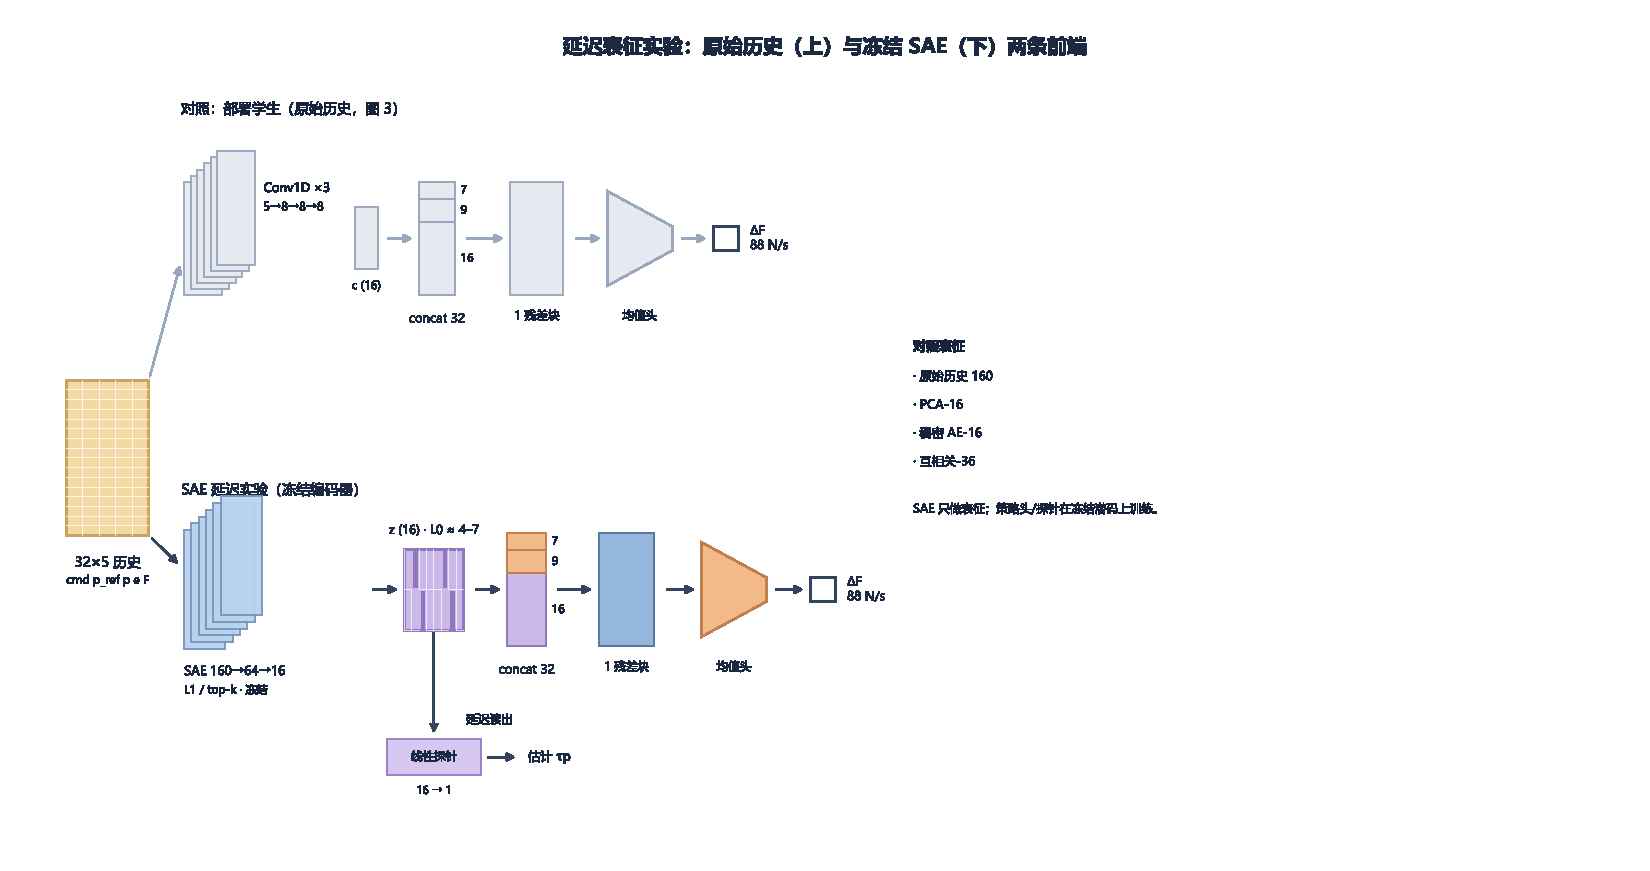
\includegraphics[width=1.00\linewidth,height=.65\textheight,keepaspectratio]{figures/fig12.pdf}
\caption{延迟表征实验的两条前端：部署学生使用原始 32\ensuremath{\times}5 历史（上）；实验分支将历史送入冻结 SAE，得到 16 维稀疏潜码，再分别接策略头或线性延迟探针（下）。SAE 只做表征，策略/探针在冻结潜码上训练；对照包括 PCA、稠密 AE、原始历史和互相关。}
\end{figure}
\hypertarget{analysis-delay-network}{}\label{analysis-delay-network}
基线历史特征和替换前端的潜码均为 16 维，主要区别在于学习目标与训练方式。基线随控制任务联合优化，PCA、AE 和 SAE 替换前端在表征学习后冻结；SAE 辅助分支则在保留基线特征时增加潜码。后续控制结果据此比较历史信息的使用方式。

\subsection{时延信息读出的完整结果}
\hypertarget{s612}{}\label{s612}
原始 tiny 学生在短、中、长延迟层的闭环通过率分别为 94.0\%、93.5\% 和 88.8\%，中位 RMSE 分别为 0.343、0.363 和 0.438 deg/s，长延迟层表现较弱。表 8 和图 13 考察这一差异对应的时延信息是否能从历史中读出。

\begin{table}[!htbp]\centering
\caption{从因果历史前缀估计 \ensuremath{\tau}\textsubscript{p} 的留出结果（120 个，960 episode）}
\small\setlength{\tabcolsep}{4pt}\renewcommand{\arraystretch}{1.18}
\begin{tabularx}{\linewidth}{>{\hsize=1\hsize\linewidth=\hsize\raggedright\arraybackslash}X>{\hsize=1\hsize\linewidth=\hsize\raggedright\arraybackslash}X>{\hsize=1\hsize\linewidth=\hsize\raggedright\arraybackslash}X>{\hsize=1\hsize\linewidth=\hsize\raggedright\arraybackslash}X>{\hsize=1\hsize\linewidth=\hsize\raggedright\arraybackslash}X>{\hsize=1\hsize\linewidth=\hsize\raggedright\arraybackslash}X}\toprule
表征 & 维度 & 1.2 s R\ensuremath{{}^2} & 1.2 s MAE (ms) & 2.0 s R\ensuremath{{}^2} & 2.0 s MAE (ms) \\
\midrule
互相关（F\textsubscript{req}—p） & 36 & 0.995 & 2.9 & 0.968 & 8.4 \\
稠密 AE & 16 & 0.608 & 32.8 & 0.656 & 29.5 \\
原始历史 & 160 & 0.567 & 34.7 & 0.588 & 33.0 \\
PCA & 16 & 0.496 & 38.3 & 0.552 & 35.4 \\
通道均值 & 5 & 0.440 & 41.5 & 0.461 & 38.8 \\
L1-SAE（L0≈7） & 16 & 0.344 & 43.6 & 0.554 & 35.5 \\
Top-k SAE（k=4） & 16 & 0.122 & 53.2 & 0.506 & 37.8 \\
L1-SAE（L0≈3.5） & 16 & 0.075 & 56.1 & 0.484 & 38.2 \\
\bottomrule\end{tabularx}\end{table}
\begin{figure}[!htbp]\centering
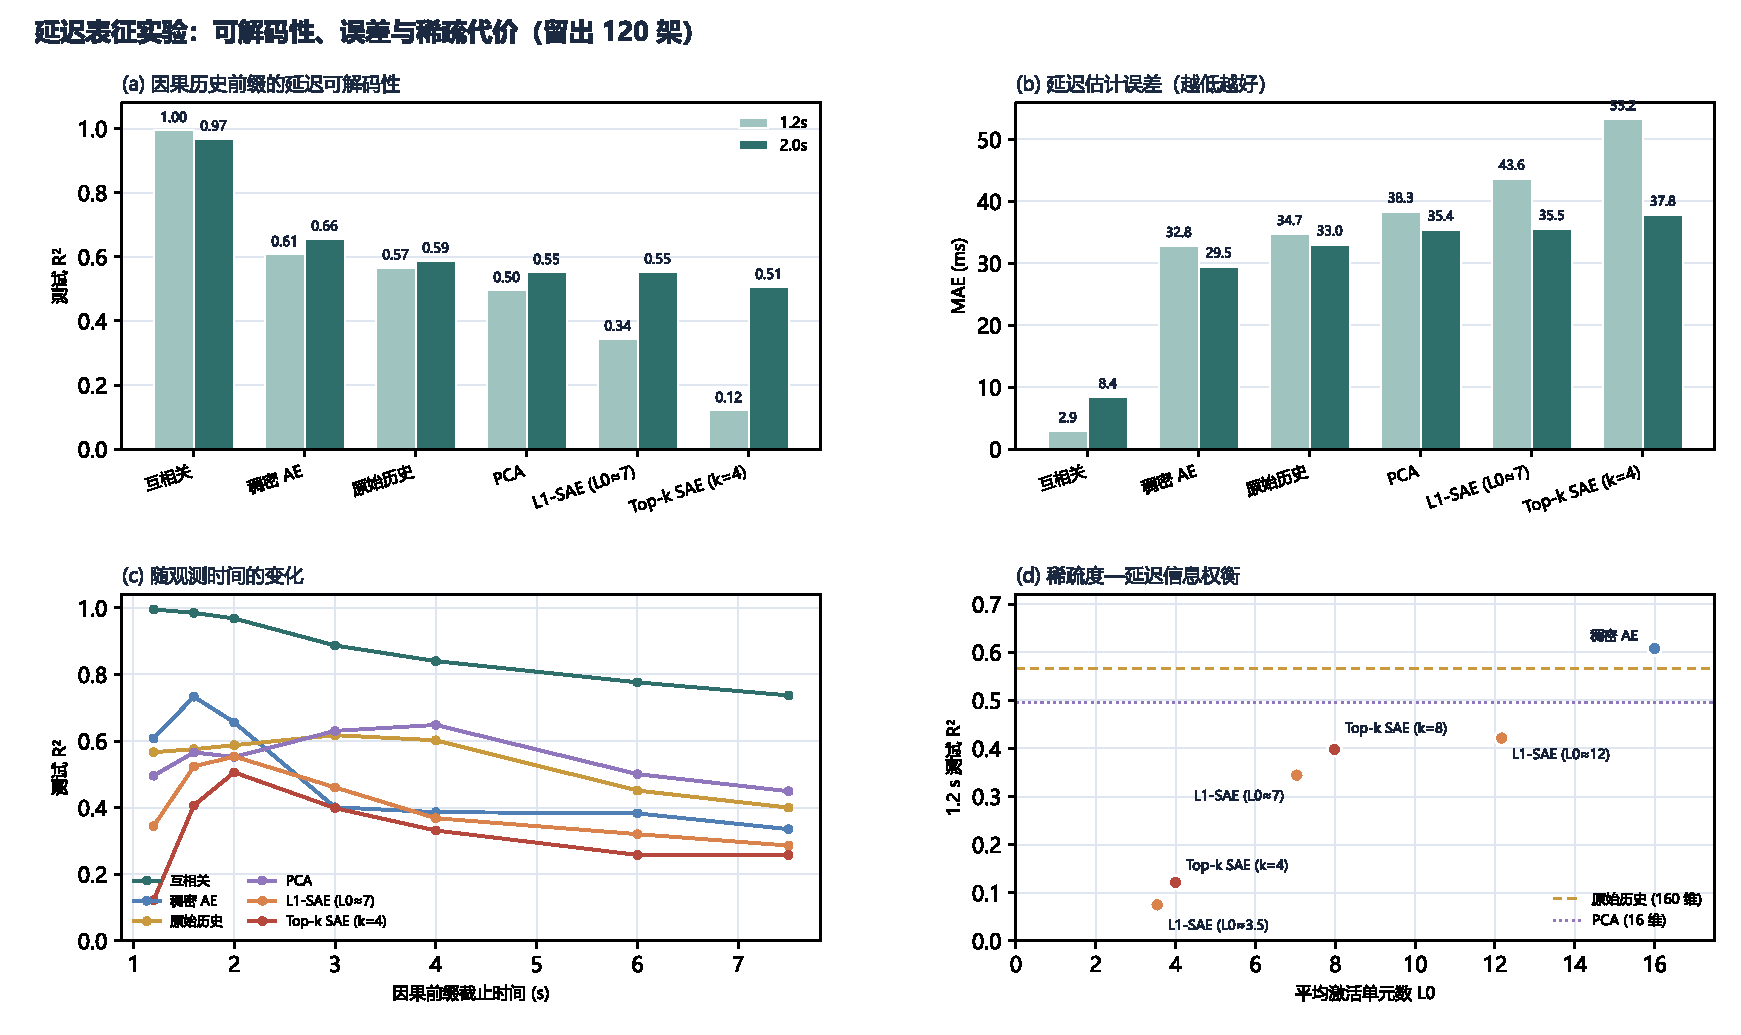
\includegraphics[width=1.00\linewidth,height=.65\textheight,keepaspectratio]{figures/fig13.pdf}
\caption{延迟表征的可解码性。(a) 1.2 s 与 2.0 s 因果前缀的测试 R\ensuremath{{}^2}；(b) 对应 MAE；(c) R\ensuremath{{}^2} 随观测时间的变化；(d) 稀疏度—延迟信息权衡。留出 120 个对象、960 个对象—指令 episode。}
\end{figure}
\hypertarget{analysis-delay-probe}{}\label{analysis-delay-probe}
1.2 s 前缀上，请求力—响应互相关的时延读出 R\ensuremath{{}^2} 为 0.995，MAE 为 2.9 ms，输入与响应的时移包含较清晰的时延线索。16 维稠密 AE 的 R\ensuremath{{}^2} 为 0.608，Top-k SAE 为 0.122。延长前缀后，Top-k SAE 与稠密 AE 的 R\ensuremath{{}^2} 分别为 0.506、0.656。各表征的读出结果与后续闭环对照共同用于选择学生的历史编码方式。

这一差异随观测时间变化：例如 Top-k SAE 的 R\ensuremath{{}^2} 从 1.2 s 的 0.122 升至 2.0 s 的 0.506。因而输入设计既取决于压缩方式，也取决于信息何时可用。对学生控制器而言，接下来的关键是这些表征在持续反馈中的效果，而非单独追求探针分数。

本组读出结果覆盖 510 个对象、0–0.2 s 时延范围，采用 16 维编码与线性探针。它支持使用历史获取对象动态信息，并为下一组闭环实验提供表征对照。

\subsection{历史表征的完整闭环对照}
\hypertarget{s613}{}\label{s613}
在同一 510 个对象划分上，将表征用于控制：PCA-16、稠密 AE-16 和 Top-k SAE-16 替换原始历史，SAE-aux 则保留原始历史并附加 SAE 潜码。动作标签由既有 tiny 学生产生，检验的是对已蒸馏控制能力的保留。原始历史微调分支与 SAE-aux 继承 tiny 权重；替换分支训练新的策略头。各分支先用 BC 数据训练，替换分支和 SAE-aux 再通过 DAgger 追加自身访问状态：在 96 个源域对象上以 β = 0.5 采样，合并数据后再训练 8 个 epoch。

\begin{figure}[!htbp]\centering
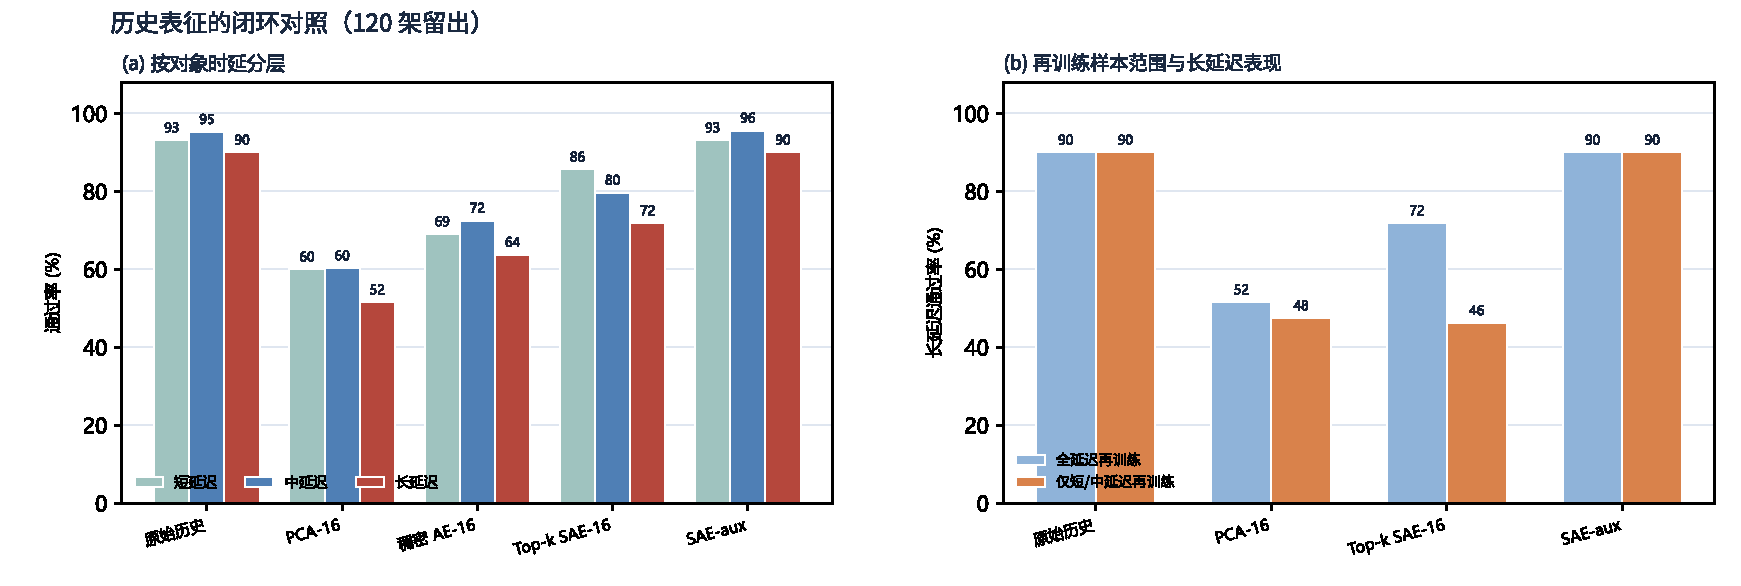
\includegraphics[width=1.00\linewidth,height=.65\textheight,keepaspectratio]{figures/fig14.pdf}
\caption{历史表征的闭环对照。左：按输入时延分层的通过率。右：全延迟样本与短/中延迟样本再训练后的长延迟表现。留出集包含 120 个对象、960 条对象—指令轨迹。}
\end{figure}
\hypertarget{analysis-delay-closed-loop}{}\label{analysis-delay-closed-loop}
保留基线时序编码的两种方案在长延迟层均通过 90.0\%，Top-k SAE、稠密 AE 和 PCA 替换方案分别为 71.9\%、63.7\%、51.6\%。将再训练数据限制为短、中时延后，Top-k SAE 的长延迟通过率降至 46.2\%，而保留基线的方案仍为 90.0\%。表征替换与训练对象覆盖共同影响了长时延控制。

\begin{table}[!htbp]\centering
\caption{历史表征的闭环性能与短/中延迟再训练对照}
\small\setlength{\tabcolsep}{4pt}\renewcommand{\arraystretch}{1.18}
\begin{tabularx}{\linewidth}{>{\hsize=1\hsize\linewidth=\hsize\raggedright\arraybackslash}X>{\hsize=1\hsize\linewidth=\hsize\raggedright\arraybackslash}X>{\hsize=1\hsize\linewidth=\hsize\raggedright\arraybackslash}X>{\hsize=1\hsize\linewidth=\hsize\raggedright\arraybackslash}X>{\hsize=1\hsize\linewidth=\hsize\raggedright\arraybackslash}X>{\hsize=1\hsize\linewidth=\hsize\raggedright\arraybackslash}X}\toprule
变体 & 短延迟 & 中延迟 & 长延迟 & 长延迟 RMSE (deg/s) & 仅短/中延迟再训练 \ensuremath{\rightarrow} 长延迟 \\
\midrule
原始历史（tiny 微调） & 93.1\% & 95.3\% & 90.0\% & 0.408 & 90.0\% \\
PCA-16 & 60.0\% & 60.3\% & 51.6\% & 1.406 & 47.5\% \\
稠密 AE-16 & 69.1\% & 72.5\% & 63.7\% & 0.731 & — \\
Top-k SAE-16 & 85.6\% & 79.7\% & 71.9\% & 0.708 & 46.2\% \\
SAE-aux（保留原始历史） & 93.1\% & 95.6\% & 90.0\% & 0.409 & 90.0\% \\
\bottomrule\end{tabularx}\end{table}
Top-k SAE 的早期时延读出分数低于稠密 AE，闭环通过率却更高。参数读出评价表征中可辨认的信息，闭环评价则反映这些信息对实际控制的作用。两类结果共同支持以控制任务表现确定历史编码方案。

在继承既有 tiny 权重的原始历史与 SAE-aux 分支中，将再训练样本限制为短、中延迟（\(\tau_{p}\) \ensuremath{\le} 0.15 s）后，长延迟留出通过率均为 90.0\%。同一限制下，PCA 为 47.5\%，Top-k SAE 为 46.2\%，后者在全延迟样本再训练时为 71.9\%。该对照比较了既定初始化下的再训练样本覆盖。

重复训练中，原始历史与 SAE-aux 的长延迟通过率保持在 90\%。PCA 与稠密 AE 各重复一次，对应范围为 51.6–55.6\% 和 52.5–63.8\%。两次比较均体现了保留基线历史编码的控制表现。

\subsection{输入时延与闭环等效延迟}
\hypertarget{s614}{}\label{s614}
闭环性能下降可能表现为滞后加大，也可能表现为持续振荡。为区分这两种情况，需要将对象输入时延 \(\tau_{p}\) 与完整受控系统的等效时间延迟 \(\tau_{e}\) 联系起来：前者在对象生成时采样，后者在控制器确定后由闭环输入输出拟合得到。同一对象采用不同控制器，可以产生不同的等效延迟。

GJB 2874-1997 A5.4.1.1.5 对滚转轴等效时间延迟的建议上限为 1 级 0.10 s、2 级 0.20 s、3 级 0.25 s（表 A21，印刷 246–247 页，PDF 250–251 页），考察前置滤波器、SAS、舵机等综合作用；A4.9（印刷 68 页，PDF 72 页）说明时间延迟项用于改善高频拟合。本文据此分析各表征策略形成的闭环动态。

拟合采用滚转轴 4 阶低阶等效系统（LOES），包含滚转、螺旋与荷兰滚模态。其分母为 (s\ensuremath{-}\ensuremath{\lambda}\textsubscript{s})(s+1/T\textsubscript{R})(s\ensuremath{{}^2}+2\ensuremath{\zeta}\textsubscript{d}\ensuremath{\omega}\textsubscript{d}s+\ensuremath{\omega}\textsubscript{d}\ensuremath{{}^2})，分子为 s(s\ensuremath{{}^2}+2\ensuremath{\zeta}\textsubscript{\ensuremath{\phi}}\ensuremath{\omega}\textsubscript{\ensuremath{\phi}}s+\ensuremath{\omega}\textsubscript{\ensuremath{\phi}}\ensuremath{{}^2})，并带有延迟项 e\textsuperscript{\ensuremath{-}\ensuremath{\tau}\textsubscript{e}s}；对应 GJB A5.4.1.1.1（印刷 210–212 页，PDF 214–216 页）的滚转速率模态结构。

两类时延在实验中的用途见表 10：\(\tau_{p}\) 用于构造对象和分层分析，\(\tau_{e}\) 用于描述控制策略形成的整体响应。对闭环频响先检查 4 阶 LOES 的拟合残差，再报告等效延迟，便可同时识别“响应滞后”和“响应已难以用该线性结构描述”两类现象。

\begin{table}[!htbp]\centering
\caption{对象输入时延与闭环等效延迟的定义及用途}
\small\setlength{\tabcolsep}{4pt}\renewcommand{\arraystretch}{1.18}
\begin{tabularx}{\linewidth}{>{\hsize=1\hsize\linewidth=\hsize\raggedright\arraybackslash}X>{\hsize=1\hsize\linewidth=\hsize\raggedright\arraybackslash}X>{\hsize=1\hsize\linewidth=\hsize\raggedright\arraybackslash}X}\toprule
项目 & \ensuremath{\tau}\textsubscript{p}（本文对象参数） & \ensuremath{\tau}\textsubscript{e}（GJB A21 评价量） \\
\midrule
数学位置 & 对象输入前 e\textsuperscript{\ensuremath{-}\ensuremath{\tau}\textsubscript{p}s} & 闭环 LOES 拟合项 e\textsuperscript{\ensuremath{-}\ensuremath{\tau}\textsubscript{e}s} \\
已知时机 & 训练前采样 & 控制器确定后拟合 \\
依赖控制器 & 否 & 是 \\
主要用途 & 对象生成、训练、延迟分层 & 飞行品质评价 \\
范围 / 门限 & 0.001–0.20 s 常态；0.5 s OOD & 1 级 \ensuremath{\le}0.10 s；2 级 \ensuremath{\le}0.20 s；3 级 \ensuremath{\le}0.25 s \\
A21 可评性 & 不可直接评 & 需拟合残差合格 \\
\bottomrule\end{tabularx}\end{table}
因此，前面的探针检验学生能否获取对象时延信息；下面的 LOES 分析则检验不同表征策略最终产生了怎样的闭环动态。二者共同服务于统一控制器的输入选择。

\subsection{长时闭环频响与 LOES 诊断}
\hypertarget{s615}{}\label{s615}
在 120 个留出对象（短、中、长各 40 个）上，对原始历史、Top-k SAE-16 和 SAE-aux 注入 0.1–10 rad/s 的 18 分量多正弦滚转指令，记录 180 s 闭环响应。以 50 Hz 输入输出估计 H(j\ensuremath{\omega}) = P/P\textsubscript{c}，再拟合 4 阶滚转 LOES 和 \(\tau_{e}\)，沿用各策略既有闭环及其记录信号。

以幅值 VAF \ensuremath{\ge} 0.95、相位 RMSE \ensuremath{\le} 10° 作为本实验的拟合门限。通过拟合门的对象按 A21 延迟阈值分档，其余单列为未通过拟合。表 11 和图 15 同时报告可评数和等效延迟分布。

\begin{table}[!htbp]\centering
\caption{不同历史表征策略的闭环 LOES 拟合与等效延迟}
\small\setlength{\tabcolsep}{4pt}\renewcommand{\arraystretch}{1.18}
\begin{tabularx}{\linewidth}{>{\hsize=1.5\hsize\linewidth=\hsize\raggedright\arraybackslash}X>{\hsize=1.05\hsize\linewidth=\hsize\raggedright\arraybackslash}X>{\hsize=1.2\hsize\linewidth=\hsize\raggedright\arraybackslash}X>{\hsize=1.85\hsize\linewidth=\hsize\raggedright\arraybackslash}X>{\hsize=0.6\hsize\linewidth=\hsize\raggedright\arraybackslash}X>{\hsize=0.6\hsize\linewidth=\hsize\raggedright\arraybackslash}X>{\hsize=0.6\hsize\linewidth=\hsize\raggedright\arraybackslash}X>{\hsize=0.6\hsize\linewidth=\hsize\raggedright\arraybackslash}X}\toprule
策略 & 可评 / 120 & \ensuremath{\tau}\textsubscript{e} 中位 (s) & 短 / 中 / 长中位 (s) & 1 级 & 2 级 & 3 级 & >3 级 \\
\midrule
原始历史 & 73/120 & 0.073 & 0.042 / 0.127 / 0.299 & 43 & 15 & 4 & 11 \\
SAE-aux & 102/120 & 0.102 & 0.032 / 0.125 / 0.309 & 51 & 14 & 7 & 30 \\
Top-k SAE-16 & 0/120 & — & — / — / — & 0 & 0 & 0 & 0 \\
\bottomrule\end{tabularx}\end{table}
\begin{figure}[!htbp]\centering
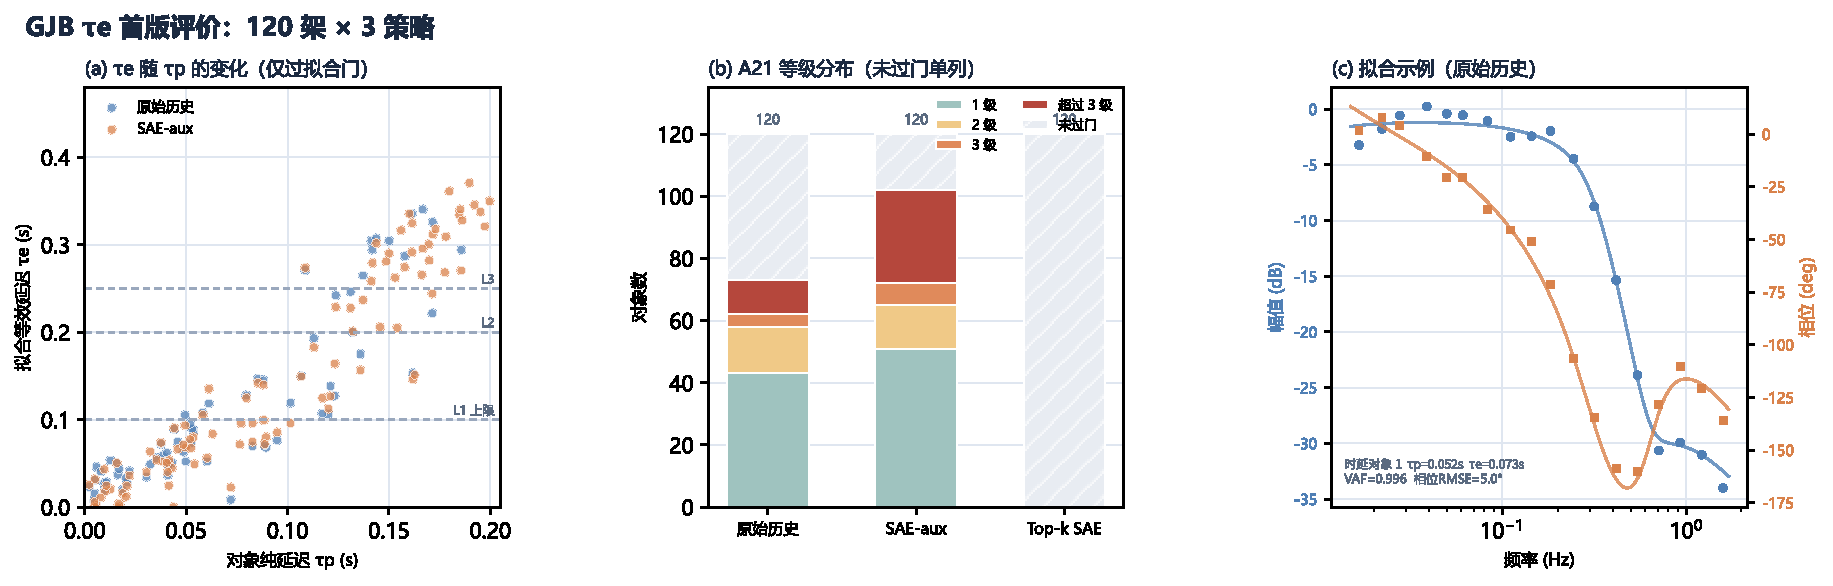
\includegraphics[width=1.00\linewidth,height=.65\textheight,keepaspectratio]{figures/fig15.pdf}
\caption{不同历史表征策略的闭环等效延迟。(a) 可评对象的 \ensuremath{\tau}e 与 \ensuremath{\tau}p；(b) A21 等级分布（未过拟合门的对象单列）；(c) 一个原始历史对象的 Bode 拟合示例。Top-k SAE-16 的 120 个全部未过拟合门，因此没有 A21 等级。}
\end{figure}
\hypertarget{analysis-tau-e-eval}{}\label{analysis-tau-e-eval}
原始历史与 SAE-aux 在长时延层的可评等效延迟约为 0.30 s，高于本文采用的三级建议上限 0.25 s。两者分别有 73、102 个对象通过拟合门，Top-k SAE 为 0/120。总体中位数对应不同的可评对象集合，控制器间的延迟差异还需结合共同对象及拟合残差解释。

更明显的差异出现在 Top-k SAE-16：原始历史有 73/120 个通过拟合，SAE-aux 有 102/120 个，Top-k SAE 为 0/120。其 VAF 中位为 0.824、相位 RMSE 中位为 35.1°。结合图 18 的 180 s 响应和功率谱，可见持续低频振荡；这一变化超出了单一延迟数值所能描述的范围。

通过拟合门的对象中，原始历史按 1、2、3、超过 3 级阈值分档的数量为 43、15、4、11，SAE-aux 为 51、14、7、30。SAE-aux 的可评集合更大，因而两组总体中位数 0.073 s 与 0.102 s 对应不同对象集合；比较控制器的延迟差异还需考察共同可评对象。

由此，闭环表征的判断需要同时看短时跟踪、长时振荡和频域拟合。SAE-aux 保留了原始历史的短时通过率，并提高了 LOES 可评数；Top-k SAE 直接替换历史后，则暴露出短时统计未充分体现的长时动态问题。下面检查这一现象对激励幅值与训练重复是否稳定。

\subsection{激励幅值与训练重复检查}
\hypertarget{s616}{}\label{s616}
首先在同一 120 个对象、3 种策略上，将多正弦每分量幅值设为 0.5、1.0、2.0 deg/s，保持拟合协议与门限一致。表 12 和图 16 同时比较可评数及三档幅值共同可评对象上的等效延迟。

\begin{table}[!htbp]\centering
\caption{激励幅值对 \ensuremath{\tau}\textsubscript{e} 评价的影响（120 个 \ensuremath{\times} 3 策略）}
\small\setlength{\tabcolsep}{4pt}\renewcommand{\arraystretch}{1.18}
\begin{tabularx}{\linewidth}{>{\hsize=1\hsize\linewidth=\hsize\raggedright\arraybackslash}X>{\hsize=1\hsize\linewidth=\hsize\raggedright\arraybackslash}X>{\hsize=1\hsize\linewidth=\hsize\raggedright\arraybackslash}X>{\hsize=1\hsize\linewidth=\hsize\raggedright\arraybackslash}X>{\hsize=1\hsize\linewidth=\hsize\raggedright\arraybackslash}X}\toprule
策略 & 可评 / 120（0.5 / 1.0 / 2.0） & \ensuremath{\tau}\textsubscript{e} 中位（0.5 / 1.0 / 2.0） & 共同可评 n & 共同集 \ensuremath{\tau}\textsubscript{e} 范围 (s) \\
\midrule
原始历史 & 41 / 73 / 91 & 0.065 / 0.073 / 0.094 & 40 & 0.055–0.066 \\
SAE-aux & 78 / 102 / 111 & 0.111 / 0.102 / 0.127 & 75 & 0.105–0.116 \\
Top-k SAE-16 & 0 / 0 / 0 & — / — / — & 0 & — \\
\bottomrule\end{tabularx}\end{table}
\begin{figure}[!htbp]\centering
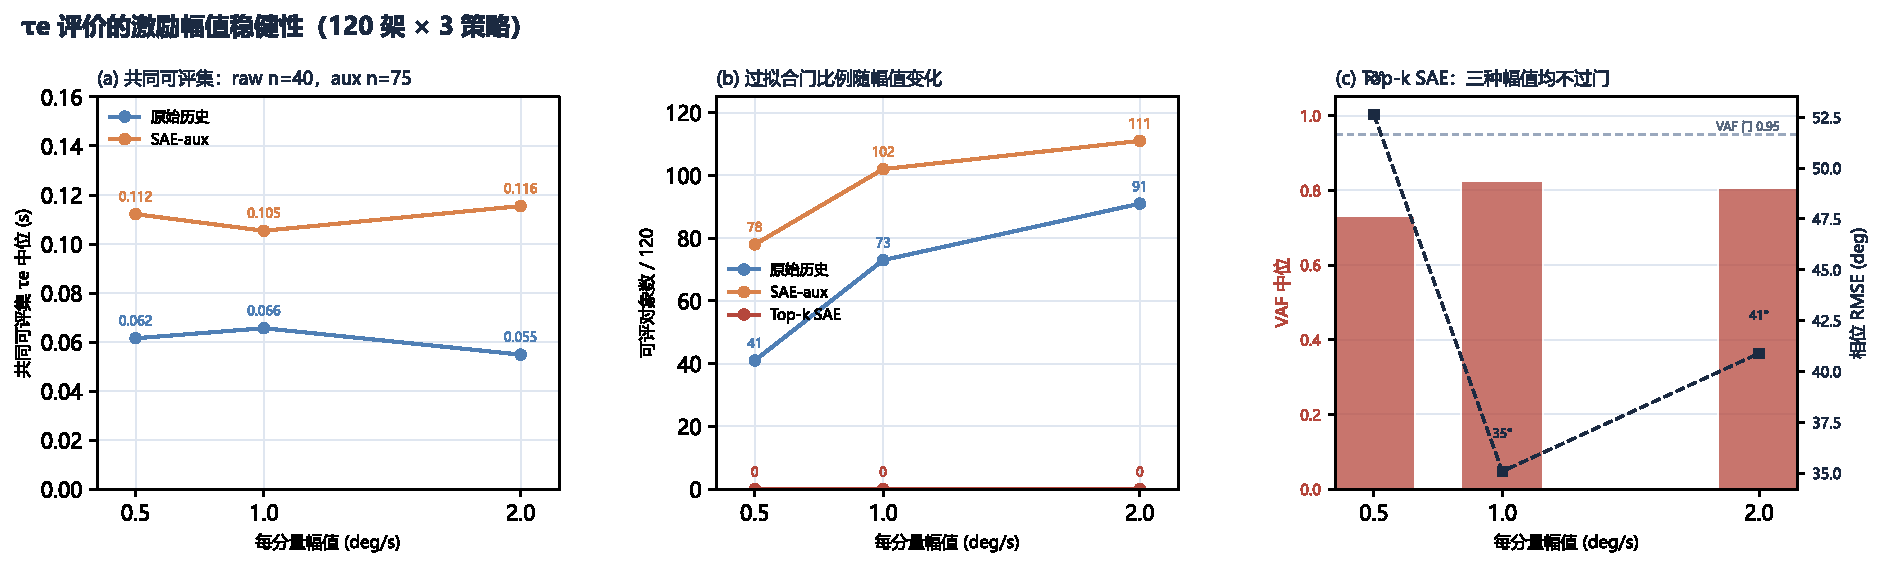
\includegraphics[width=1.00\linewidth,height=.65\textheight,keepaspectratio]{figures/fig16.pdf}
\caption{\ensuremath{\tau}e 评价的激励幅值稳健性。(a) 三种幅值共同可评对象上的 \ensuremath{\tau}e 中位；(b) 可评对象数随幅值变化；(c) Top-k SAE 在三种幅值下的 VAF 与相位残差。}
\end{figure}
\hypertarget{analysis-tau-e-amplitude}{}\label{analysis-tau-e-amplitude}
激励幅值增加时，原始历史的可评对象数由 41 增至 91，SAE-aux 由 78 增至 111。在三档幅值共同可评的对象上，等效延迟中位数分别保持在 0.055–0.066 s 和 0.105–0.116 s。幅值对纳入统计的对象数影响较大，共同对象上的延迟量级变化较小。

Top-k SAE-16 在三档幅值下均为 0/120 可评，VAF 中位分别为 0.732、0.824、0.807，相位 RMSE 中位分别为 52.6°、35.1°、40.9°。改变激励幅值后，其闭环响应仍难以由当前 4 阶 LOES 描述。

将相位门限取为 8°、10°、12°，原始历史可评数为 53、73、84，\(\tau_{e}\) 中位为 0.071、0.073、0.090 s；SAE-aux 为 81、102、110 个和 0.100、0.102、0.098 s；Top-k SAE 均为 0。门限影响纳入统计的对象数，但上述动态差异保持一致。

其次，三种策略各用第二种子按原 BC/DAgger 配置训练，再进行同一闭环评价，结果见表 13 和图 17。

\begin{table}[!htbp]\centering
\caption{策略种子对 \ensuremath{\tau}\textsubscript{e} 评价的影响（120 个）}
\small\setlength{\tabcolsep}{4pt}\renewcommand{\arraystretch}{1.18}
\begin{tabularx}{\linewidth}{>{\hsize=1\hsize\linewidth=\hsize\raggedright\arraybackslash}X>{\hsize=1\hsize\linewidth=\hsize\raggedright\arraybackslash}X>{\hsize=1\hsize\linewidth=\hsize\raggedright\arraybackslash}X>{\hsize=1\hsize\linewidth=\hsize\raggedright\arraybackslash}X>{\hsize=1\hsize\linewidth=\hsize\raggedright\arraybackslash}X>{\hsize=1\hsize\linewidth=\hsize\raggedright\arraybackslash}X}\toprule
策略 & 可评（s1 / s2） & \ensuremath{\tau}\textsubscript{e} 中位（s1 / s2） & 共同 n & 共同中位（s1 / s2） & 1/2/3/>3 级（s1 \ensuremath{\rightarrow} s2） \\
\midrule
原始历史 & 73 / 77 & 0.073 / 0.078 & 73 & 0.073 / 0.075 & 43/15/4/11 \ensuremath{\rightarrow} 43/15/5/14 \\
SAE-aux & 102 / 106 & 0.102 / 0.106 & 101 & 0.100 / 0.095 & 51/14/7/30 \ensuremath{\rightarrow} 52/15/7/32 \\
Top-k SAE-16 & 0 / 0 & — / — & 0 & — & 0/0/0/0 \ensuremath{\rightarrow} 0/0/0/0 \\
\bottomrule\end{tabularx}\end{table}
\begin{figure}[!htbp]\centering
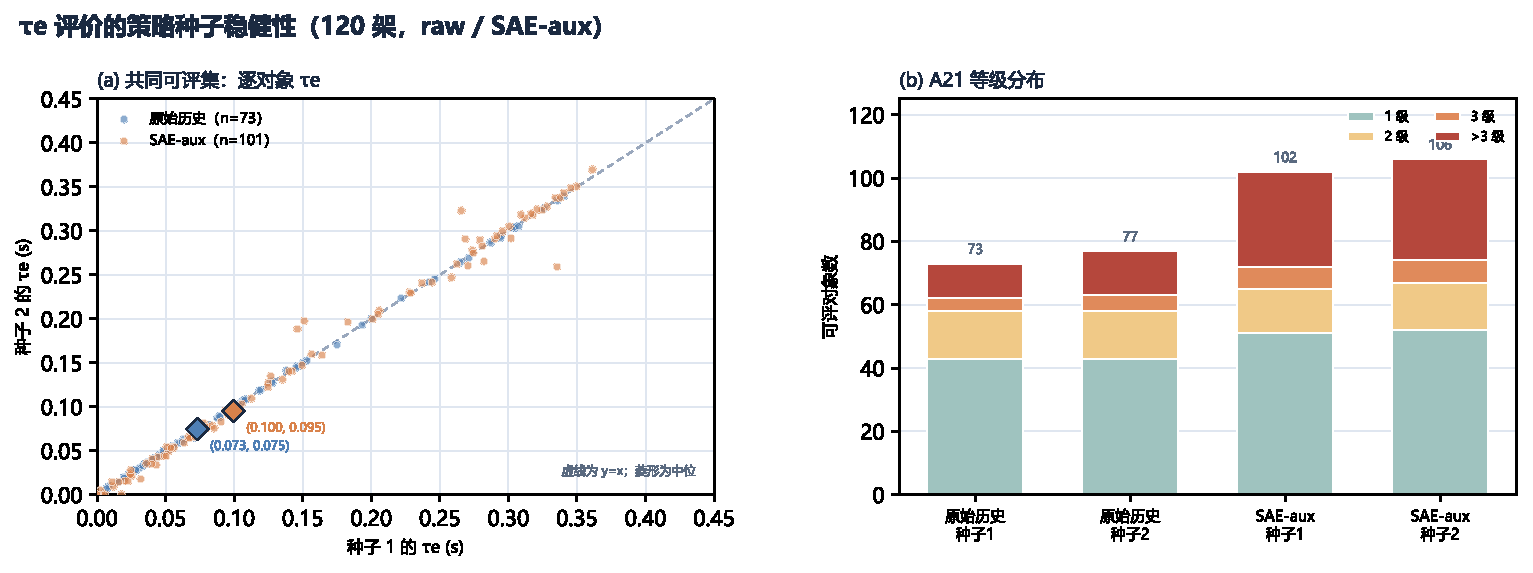
\includegraphics[width=1.00\linewidth,height=.65\textheight,keepaspectratio]{figures/fig17.pdf}
\caption{\ensuremath{\tau}e 评价的策略种子稳健性。(a) 两个种子共同可评对象的逐对象 \ensuremath{\tau}e；(b) 两个种子的 A21 等级分布。}
\end{figure}
\hypertarget{analysis-tau-e-seed}{}\label{analysis-tau-e-seed}
第二个种子下，原始历史的可评对象数由 73 变为 77，SAE-aux 由 102 变为 106。共同对象上的延迟中位数分别为 0.073/0.075 s、0.100/0.095 s，Top-k SAE 两个种子均无可评对象。这两次重复中，各表征方案的主要动态差异保持一致。

图 18 给出同一时延对象上的长时响应与功率谱。

\begin{figure}[!htbp]\centering
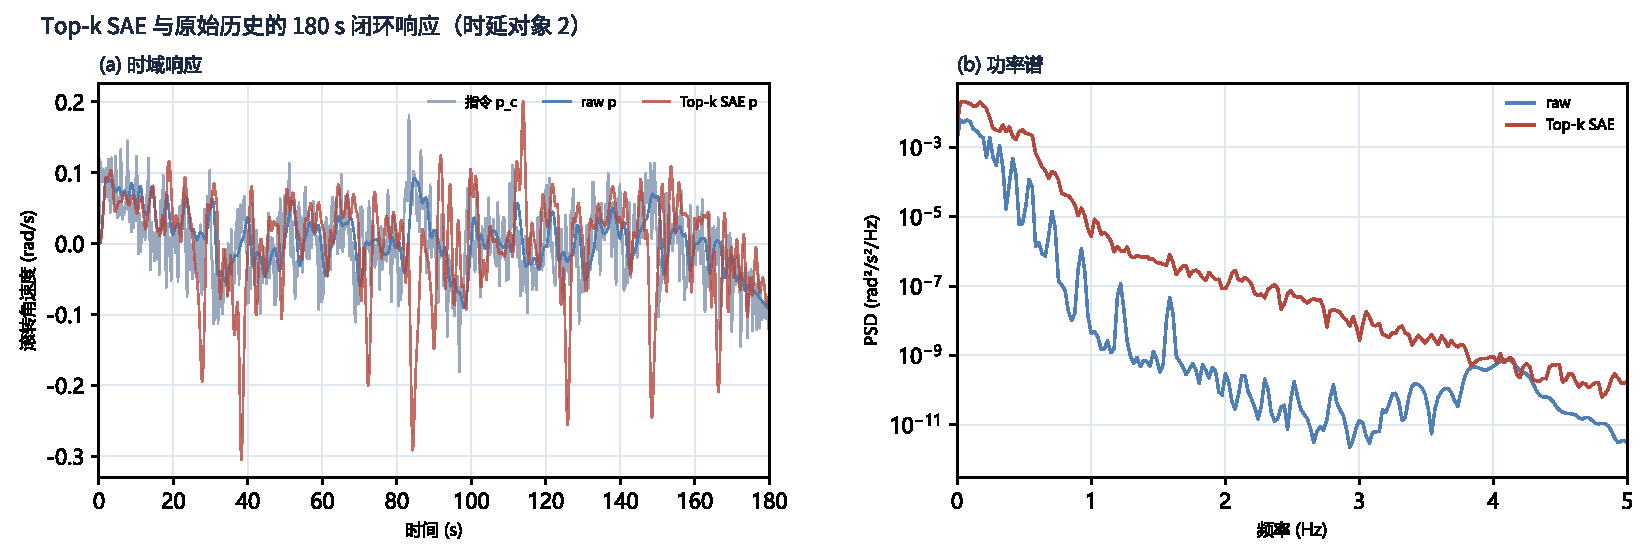
\includegraphics[width=1.00\linewidth,height=.65\textheight,keepaspectratio]{figures/fig18.pdf}
\caption{Top-k SAE 与原始历史的 180 s 闭环响应（时延对象 2，每分量 1 deg/s）。左：时域响应；右：功率谱。Top-k SAE 的低频功率较高，对应持续低频摆动与较大的 LOES 拟合残差。}
\end{figure}
\hypertarget{analysis-topk4-diagnostic}{}\label{analysis-topk4-diagnostic}
相同激励下，Top-k SAE 分支在 180 s 内仍有持续摆动，低频段功率也高于原始历史分支。这一响应形态与其较大的频域拟合残差相对应。短时误差统计以外，长时曲线进一步显示了替换历史表征后出现的低频动态变化。

\FloatBarrier
\section{对象分布与控制器补充结果}
\hypertarget{appendix-results}{}\label{appendix-results}
\subsection{对象分布与教师学习诊断}
\hypertarget{results-distribution-details}{}\label{results-distribution-details}
图中给出八项对象参数的边际分布，配合正文的二维散点描述取值范围及其相互约束。

\begin{figure}[!htbp]\centering
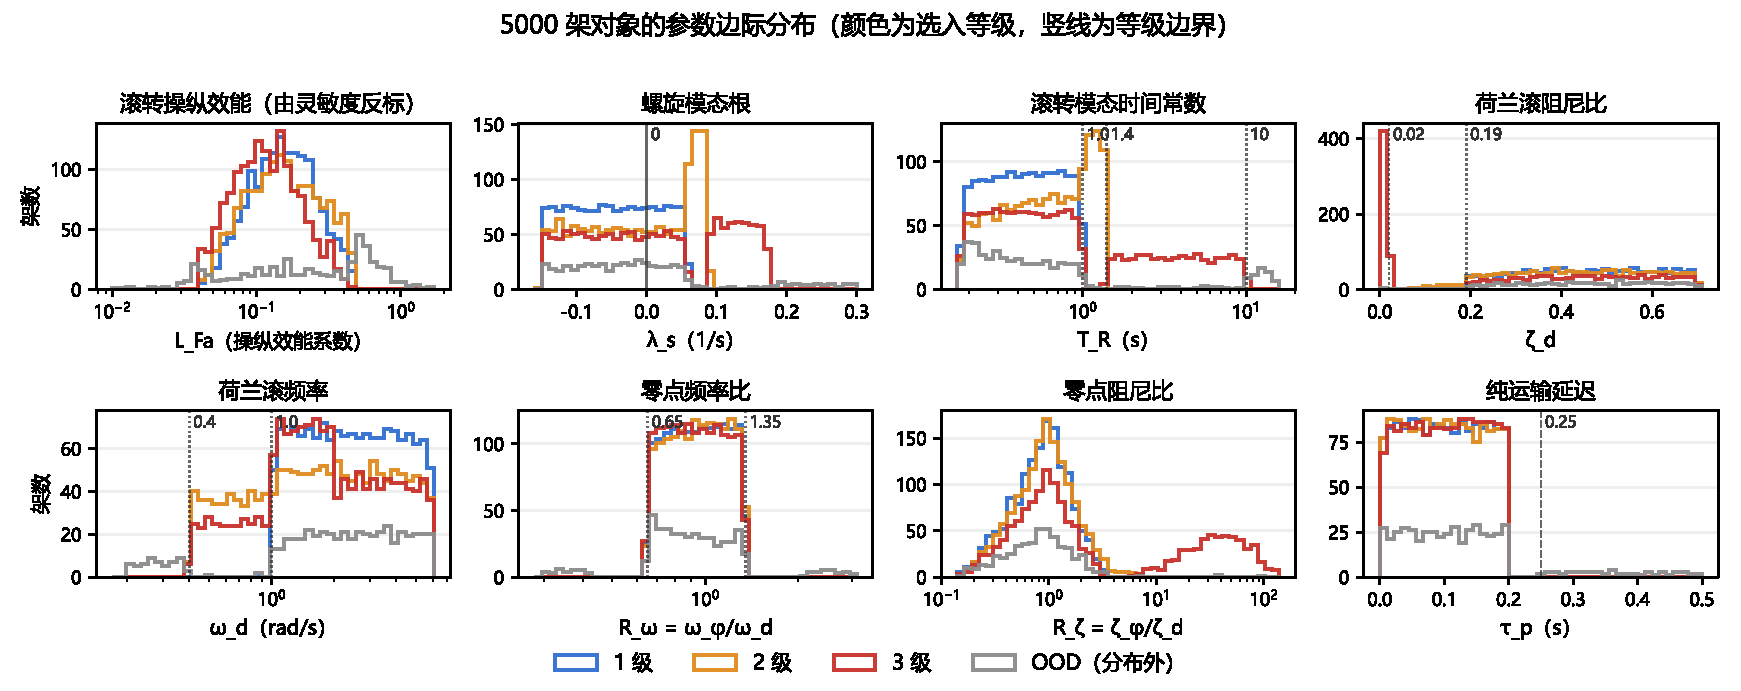
\includegraphics[width=1.00\linewidth,height=.65\textheight,keepaspectratio]{figures/fig19.pdf}
\caption{5,000 个对象的参数边际分布。颜色表示选入等级，竖线标出相应分级或研究包络边界。}
\end{figure}
\hypertarget{analysis-sampling-marginals}{}\label{analysis-sampling-marginals}
同分布对象的时延位于 0.001–0.20 s，零点频率比位于 0.65–1.35；分布外部分延伸到这些区间之外。零点阻尼比例系数的跨度较大，是由零点阻尼除以模态阻尼得到的，低阻尼候选会产生较大的比例值。操纵效能的分布则受 1 s 灵敏度标定与效能包络共同约束。

\begin{figure}[!htbp]\centering
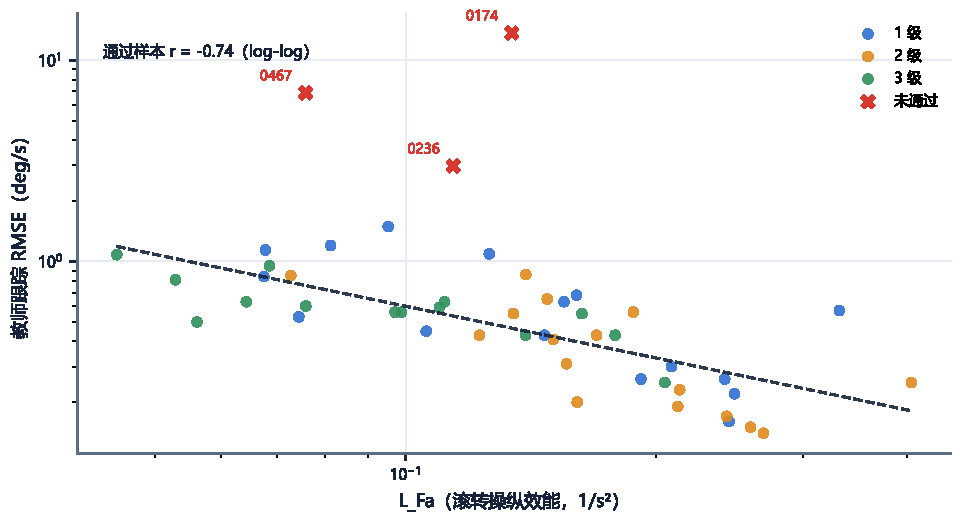
\includegraphics[width=0.70\linewidth,height=.65\textheight,keepaspectratio]{figures/fig20.pdf}
\caption{教师跟踪误差与滚转操纵效能的关系（双对数）。颜色表示品质等级，红叉表示未通过对象；虚线为通过样本的拟合，相关系数 r = \ensuremath{-}0.74。}
\end{figure}
\hypertarget{analysis-teacher-difficulty}{}\label{analysis-teacher-difficulty}
达标教师中，操纵效能与跟踪 RMSE 的双对数相关系数为 \ensuremath{-}0.74，较低效能一侧的误差总体更大，未通过样例也集中在该区域。在当前力接口和训练设置下，低效能对象是误差较突出的部分；相近效能处仍有分散，其他模态和时延条件也随对象变化。

\begin{figure}[!htbp]\centering
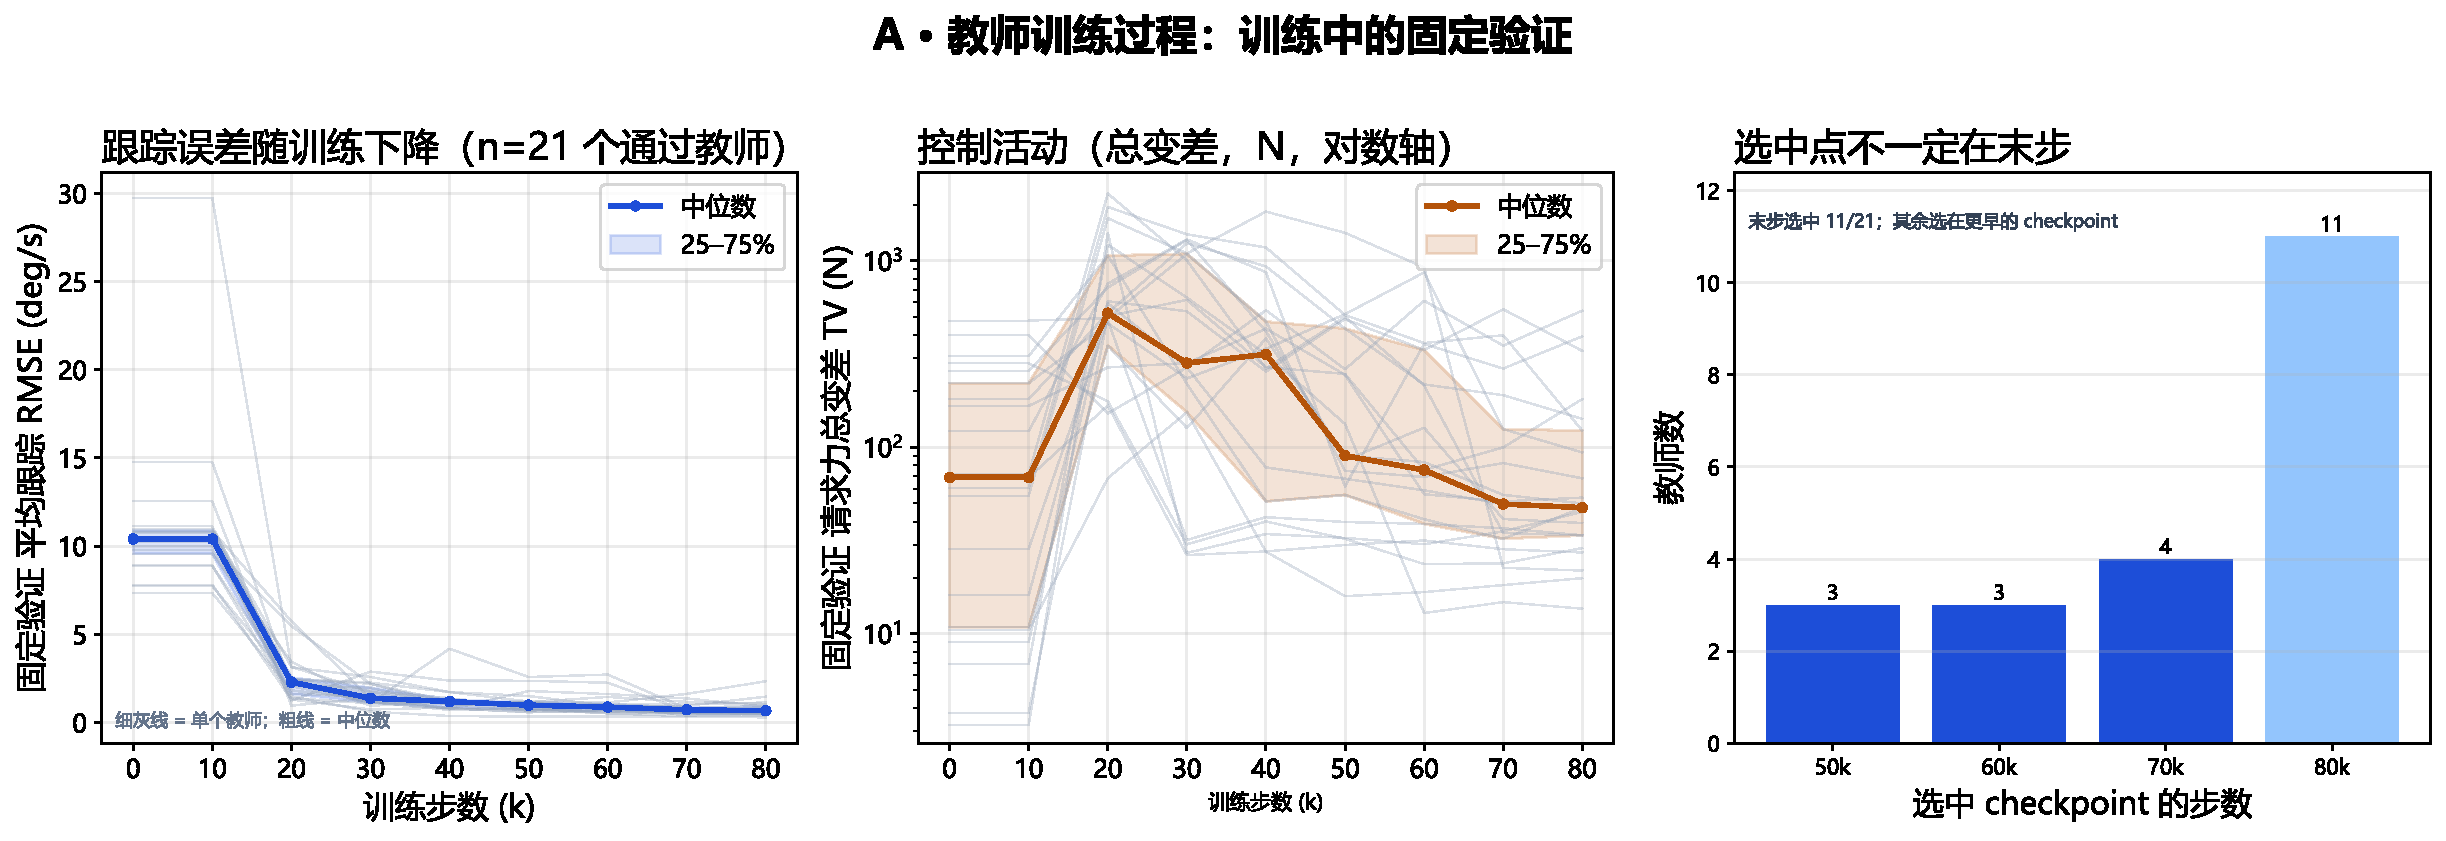
\includegraphics[width=1.00\linewidth,height=.65\textheight,keepaspectratio]{figures/fig21.pdf}
\caption{21 个达标教师的固定指令集验证结果：跟踪误差、操纵总变差及所选权重对应的训练步数。}
\end{figure}
\hypertarget{analysis-teacher-training-curves}{}\label{analysis-teacher-training-curves}
固定验证误差随训练总体下降，请求力总变差则呈现不同的变化过程。21 个存档教师中，11 个选择最后一个检查点，其余 10 个选择更早的权重。最终选用的控制器由验证表现确定，训练末步与所选权重并不总是相同。

\subsection{目标域逐状态结果与模型规模对照}
\hypertarget{results-transfer-details}{}\label{results-transfer-details}
small 学生在 12 个 DHC-6 辨识模型上的逐状态更新结果如下；8 个状态用于适配，4 个状态用于留出评价。两张表分别汇总 small 的状态分组结果及 tiny、small 的模型规模对照。

\begin{figure}[!htbp]\centering
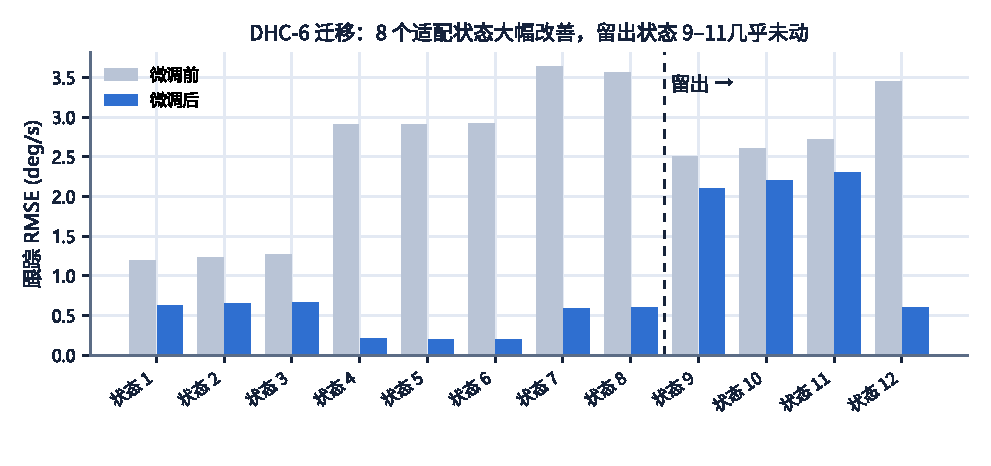
\includegraphics[width=0.88\linewidth,height=.65\textheight,keepaspectratio]{figures/fig22.pdf}
\caption{DHC-6 仿真 ARX 对象上的微调前后对照（15 deg/s 阶跃）；虚线区分适配与留出状态。}
\end{figure}
\hypertarget{analysis-dhc6-transfer}{}\label{analysis-dhc6-transfer}
逐状态结果显示更新效果随配平状态变化：状态 12 的误差下降较明显，状态 9–11 的残余误差较大。留出组的中位误差与各状态的时域响应共同描述跨状态复用，并将振荡减弱和最终目标偏差区分开来。

\begin{table}[!htbp]\centering
\hypertarget{dhc6-adaptation-summary}{}\label{dhc6-adaptation-summary}
\caption{DHC-6 仿真微调前后跟踪误差（中位数）}
\small\setlength{\tabcolsep}{4pt}\renewcommand{\arraystretch}{1.18}
\begin{tabularx}{\linewidth}{>{\hsize=1\hsize\linewidth=\hsize\raggedright\arraybackslash}X>{\hsize=1\hsize\linewidth=\hsize\raggedright\arraybackslash}X>{\hsize=1\hsize\linewidth=\hsize\raggedright\arraybackslash}X>{\hsize=1\hsize\linewidth=\hsize\raggedright\arraybackslash}X>{\hsize=1\hsize\linewidth=\hsize\raggedright\arraybackslash}X}\toprule
状态组 & 样本数 & 微调前 RMSE（deg/s） & 微调后 RMSE（deg/s） & 相对变化 \\
\midrule
适配 & 8 & 2.913 & 0.595 & 下降 79.6\% \\
留出 & 4 & 2.662 & 2.148 & 下降 19.3\% \\
\bottomrule\end{tabularx}\end{table}
\begin{table}[!htbp]\centering
\hypertarget{dhc6-capacity-comparison}{}\label{dhc6-capacity-comparison}
\caption{两种容量学生在 DHC-6 上的微调前后（中位 RMSE，deg/s）}
\small\setlength{\tabcolsep}{4pt}\renewcommand{\arraystretch}{1.18}
\begin{tabularx}{\linewidth}{>{\hsize=1\hsize\linewidth=\hsize\raggedright\arraybackslash}X>{\hsize=1\hsize\linewidth=\hsize\raggedright\arraybackslash}X>{\hsize=1\hsize\linewidth=\hsize\raggedright\arraybackslash}X>{\hsize=1\hsize\linewidth=\hsize\raggedright\arraybackslash}X>{\hsize=1\hsize\linewidth=\hsize\raggedright\arraybackslash}X>{\hsize=1\hsize\linewidth=\hsize\raggedright\arraybackslash}X}\toprule
学生 & 参数量 & 适配前 & 适配后 & 留出前 & 留出后 \\
\midrule
tiny & 3,856 & 4.127 & 1.574 & 2.778 & 2.624 \\
small & 75,040 & 2.913 & 0.595 & 2.662 & 2.148 \\
\bottomrule\end{tabularx}\end{table}
相同微调设置下，tiny 学生的适配后 RMSE 为 1.57 deg/s，small 为 0.59 deg/s，相差约 2.7 倍；源域蒸馏的中位比相应为 1.28 和 1.34。两档网络分别提供轻量共享策略与较大参数容量的实现选择，small 在本组目标域更新中取得更高跟踪精度。40 次更新中，每个适配状态被访问 5 次，构成该比较的共同更新预算。

\subsection{固定增益 PID 对照}
\hypertarget{results-pid-comparison}{}\label{results-pid-comparison}
\hypertarget{s534}{}\label{s534}
在 300 个同分布对象和 500 个分布外对象上，比较统一学生与固定增益二自由度 PID。300 个同分布对象从主试验 48 个评估对象之外抽取；两者采用相同的 14 条输入配置与控制接口，每个对象—指令组合重复两次。学生权重与 PID 增益在扫描期间保持固定。

在相同的 300 个同分布对象、500 个分布外对象及指令配置上，以固定增益二自由度 PID 为对照。PID 含参考前馈和抗积分饱和，采用相同的 \ensuremath{\pm}22 N 请求力范围及力速率接口。增益在主试验对象 7 上通过网格搜索确定，取 \(k_{p}\) = 128、\(k_{i}\) = 60、\(k_{d}\) = 0.8、\(k_{ff}\) = 6.0，随后在全部对象上保持固定。

\begin{table}[!htbp]\centering
\hypertarget{pid-student-comparison}{}\label{pid-student-comparison}
\caption{固定增益 PID 与统一学生在同一批对象上的对照。阶跃行括号内为 RMSE 中位数（deg/s）。}
\small\setlength{\tabcolsep}{4pt}\renewcommand{\arraystretch}{1.18}
\begin{tabularx}{\linewidth}{>{\hsize=1\hsize\linewidth=\hsize\raggedright\arraybackslash}X>{\hsize=1\hsize\linewidth=\hsize\raggedright\arraybackslash}X>{\hsize=1\hsize\linewidth=\hsize\raggedright\arraybackslash}X>{\hsize=1\hsize\linewidth=\hsize\raggedright\arraybackslash}X>{\hsize=1\hsize\linewidth=\hsize\raggedright\arraybackslash}X}\toprule
指令 & PID·同分布 & 学生·同分布 & PID·分布外 & 学生·分布外 \\
\midrule
\ensuremath{\pm}1 deg/s & 80.0\% (0.06) & 99.7\% (0.11) & 46.6\% (8.78) & 86.8\% (0.21) \\
\ensuremath{\pm}5 deg/s & 76.7\% (0.30) & 99.3\% (0.32) & 43.4\% (13.41) & 73.4\% (0.69) \\
\ensuremath{\pm}10 deg/s & 74.7\% (0.61) & 99.3\% (0.36) & 40.2\% (14.11) & 66.0\% (0.95) \\
\ensuremath{\pm}21 deg/s & 58.3\% (1.28) & 86.0\% (0.69) & 28.6\% (15.67) & 42.0\% (2.03) \\
\ensuremath{\pm}31 deg/s & 35.7\% (1.90) & 60.3\% (1.13) & 16.2\% (18.53) & 27.6\% (2.93) \\
双脉冲 / 多正弦 & 72.3\% / 78.3\% & 99.0\% / 99.7\% & 36.8\% / 43.2\% & 76.8\% / 84.4\% \\
\bottomrule\end{tabularx}\end{table}

\FloatBarrier
\end{document}
